\documentclass{scrbook}
\usepackage{graphicx} % Required for inserting images
\usepackage{tabularx} % Required for fixed width tables
\usepackage{scrlayer-scrpage} % Required for the subtitles
\usepackage{url} % Required for the URLs
\usepackage{hyperref} % Required for the URLs
\usepackage{listings} % Required for the code snippets
\usepackage{mathtools} % Required for the system of equations
\usepackage{enumitem} % Required for list styling

\usepackage{fontspec}
\setmonofont{DejaVu Sans Mono} % Overleaf has this font pre-installed

% Put the caption of the snippets at the bottom
\lstset{
	captionpos=b,
	basicstyle=\ttfamily\small,
	columns=fullflexible,
	keepspaces=true
}


\title{Hypertext Transfer Protocol Version 2 (HTTP/2, RFC 7540)}
\subtitle{Ambient intelligence course (A.Y. 2025/2026)\\Topic taught by Prof. Floriano Scioscia}
\author{Gabriele Colapinto}
\date{\today}

\begin{document}
	
	\maketitle
	\thispagestyle{empty}
	
	{\Large\textbf{License}} \\
	{Notes from Ambient intelligence (A.Y. 2025/2026) by Gabriele Colapinto. 
		Course taught by professors Michele Ruta, Floriano Scioscia, Arnaldo Tomasino, Davide Loconte — 
		Licensed under CC BY-NC 4.0.\\
		\url{https://creativecommons.org/licenses/by-nc/4.0/}}
	
	\vspace*{\fill}
	\rule{\textwidth}{0.2pt}
	\small{© 2025 Gabriele Colapinto \\
		Released under the \href{https://creativecommons.org/licenses/by-nc/4.0/}{Creative Commons Attribution–NonCommercial 4.0 International License}}
	
	\clearpage
	
	\tableofcontents

\chapter{HTTP/2: Motivation, Evolution, and Compatibility}

\section{Limits of HTTP/1.1}

HTTP/2 was introduced to address performance limitations that became increasingly relevant as web applications evolved from mostly static documents into pages composed of many heterogeneous resources. A modern page typically requires the transfer of an HTML document, style sheets, scripts, images, icons, fonts, and other auxiliary objects. Under HTTP/1.x, this resource model interacts poorly with the protocol design, because the protocol was originally optimized for simplicity rather than for efficient use of the network.\\

A first limitation is the textual representation of HTTP/1.x messages. Header fields are transmitted as plain text and are not compressed at the HTTP layer. This makes the protocol easy to inspect and implement, but it increases network traffic, especially when many requests repeat similar fields such as cookies, user-agent information, accepted media types, caching metadata, and connection-related directives.\\

A second limitation is the need for multiple connections to obtain concurrency. HTTP/1.0 effectively required a separate TCP connection for each request-response exchange. HTTP/1.1 improved this model by introducing persistent connections and request pipelining, but these mechanisms did not provide full concurrency. In practice, clients opened several parallel TCP connections to the same server in order to reduce latency and avoid waiting for resources sequentially. This strategy reduced waiting time for the client, but it increased resource consumption at both endpoints. On the server side, the cost of connection management must be multiplied by the number of simultaneous clients and by the number of concurrent connections opened by each client.\\

A third limitation is the absence of explicit resource prioritization. A browser often knows that some resources are more important for rendering or interaction than others: for instance, the main HTML document and critical style sheets usually have a stronger impact on the perceived loading time than non-critical images. HTTP/1.x does not provide a protocol-level mechanism through which the client can express these preferences to the server. As a consequence, the available TCP connection capacity can be used in an order that is not aligned with the rendering needs of the page.\\

Finally, HTTP/1.x supports only the basic request-response interaction model. The server cannot proactively send a resource merely because it knows that the client will need it. Even when the server can infer that a style sheet, script, or image is associated with the requested page, it must wait until the client discovers that dependency and sends a separate request. This introduces additional latency in the critical path of page construction.

\section{From HTTP/1.1 to HTTP/2}

HTTP/1.1 was standardized in 1997 in RFC 2068. For several years, web performance issues were mitigated through incremental improvements, implementation strategies, and application-level practices rather than through a fundamental redesign of HTTP. The most influential experimental step toward such a redesign was SPDY, announced by Google in November 2009 as a protocol intended to improve HTTP/1.1 performance.\\

By August 2012, SPDY support had appeared in popular web servers, browsers, and websites. In November 2012, the IETF HTTP Working Group, also known as \texttt{httpbis}, started from SPDY and involved its creators in the production of the first draft of the HTTP/2 specification. The design effort therefore did not begin from an abstract replacement of HTTP, but from a deployed performance-oriented protocol whose mechanisms had already been tested in practice.\\

The standardization process advanced quickly. In December 2014, HTTP/2.0 was presented as a Proposed Standard to the Internet Engineering Steering Group. In February 2015, it was published as an IETF proposed standard. In May 2015, two companion RFCs were published: RFC 7540, defining HTTP/2, and RFC 7541, defining HPACK, the header compression format used by HTTP/2.\\

The standardized name is \texttt{HTTP/2}, not \texttt{HTTP/2.0}. The disappearance of the minor version number is not merely cosmetic: the protocol introduces a new binary framing layer and therefore differs substantially from the HTTP/1.x wire format. By the end of 2015, most major web servers, including Apache httpd, Nginx, Microsoft IIS, and Node.js-based servers, and most major browsers, including Chrome, Opera, Firefox, Internet Explorer, Safari, Silk, and Edge, supported HTTP/2. In 2016, major content delivery networks such as Akamai, Cloudflare, and AWS CloudFront also supported it. By October 2017, HTTP/2 support had reached 18.1\% of the top ten million websites, which already represented a significant share of high-traffic web usage.

\section{Design Goals}

The primary design goal of HTTP/2 is to reduce latency. It does so by supporting full request and response multiplexing: multiple logical exchanges can progress concurrently over the same TCP connection. This removes the strict correspondence between one connection and one active request-response exchange that characterized earlier HTTP usage patterns.\\

A second goal is to minimize protocol overhead. HTTP/2 replaces the textual HTTP/1.x wire representation with a binary framing layer and compresses HTTP header fields using HPACK. The semantic content of the headers remains HTTP metadata, but the representation used on the network is more compact and better suited to efficient parsing.\\

A third goal is to support request prioritization. Since several streams can be active at the same time, the client needs a way to express which resources should be delivered earlier or given a larger share of available processing and bandwidth. HTTP/2 introduces a priority model based on stream dependencies and weights. Priority information is advisory: it communicates preferences to the server, but it does not impose a mandatory scheduling algorithm.\\

A fourth goal is to support server push. Server push extends the interaction model by allowing the server to send resources that are associated with a client request before the client explicitly requests them. This capability is useful when the server can determine that a resource will be needed as a consequence of a requested document.\\

The final and central constraint is the preservation of HTTP semantics. HTTP methods, status codes, URIs, header fields, caching rules, and the general meaning of requests and responses remain those of HTTP. HTTP/2 changes how messages are represented and transported between endpoints; it does not redefine the application semantics of the Web. This design choice allows existing web applications to run without modification, while browsers, servers, proxies, and content delivery networks update their protocol implementations.

\section{Why HTTP/2 Is Not HTTP/1.2}

The name HTTP/2 indicates a major protocol change. HTTP/2 introduces a binary framing layer that is not backward compatible with HTTP/1.x servers and clients at the wire-protocol level. An endpoint that only understands HTTP/1.x cannot parse an HTTP/2 frame sequence as if it were an HTTP/1.x message.\\

This incompatibility concerns protocol implementations, not web application logic. Web developers who rely on standard HTTP abstractions continue to use the same methods, status codes, URIs, and header semantics. The visible change is concentrated in the infrastructure: browsers, web servers, intermediaries, and other components that implement HTTP directly over transport connections must support the new framing and negotiation mechanisms.\\

The distinction is important. HTTP/2 extends HTTP/1.1 at the semantic level but replaces its message transfer format. From the perspective of a web application, an HTTP request is still an HTTP request and an HTTP response is still an HTTP response. From the perspective of a protocol stack, however, headers and bodies are no longer transmitted as one textual message. They are encoded into typed binary frames and carried inside streams over a connection.

\section{Pre-HTTP/2 Workarounds}

Before HTTP/2, the same performance goals were pursued with workarounds distributed across different layers of the system. Some optimizations operated at the transport and connection-management level, such as maintaining persistent TCP connections or opening several concurrent connections to the same origin. Others relied on companion protocols, such as WebSocket, when applications required long-lived bidirectional communication patterns not naturally supported by the classical HTTP request-response model.\\

Many optimizations were implemented directly in web applications and deployment practices. Small files could be concatenated into larger bundles in order to reduce the number of HTTP requests. Small images could be combined into image sprites and selected at the presentation layer. Resources could be distributed across multiple hostnames so that browser-imposed per-host connection limits were bypassed. These techniques often improved performance under HTTP/1.x, but they also introduced trade-offs. Concatenation and spriting reduce request overhead at the cost of less granular caching and more complex asset management. Domain sharding increases parallelism but also increases the number of connections, DNS lookups, and TLS handshakes.\\

Such solutions could not be fully satisfactory because they addressed symptoms rather than the underlying protocol model. The fundamental problem was not only that individual implementations needed tuning, but that HTTP/1.x lacked native mechanisms for multiplexing, prioritization, compact header representation, and proactive resource delivery. HTTP/2 integrates these mechanisms into the protocol itself while keeping the higher-level meaning of HTTP unchanged.

\chapter{The HTTP/2 Binary Framing Layer}

\section{Purpose of the Binary Framing Layer}

\begin{figure}[!h]
	\centering
	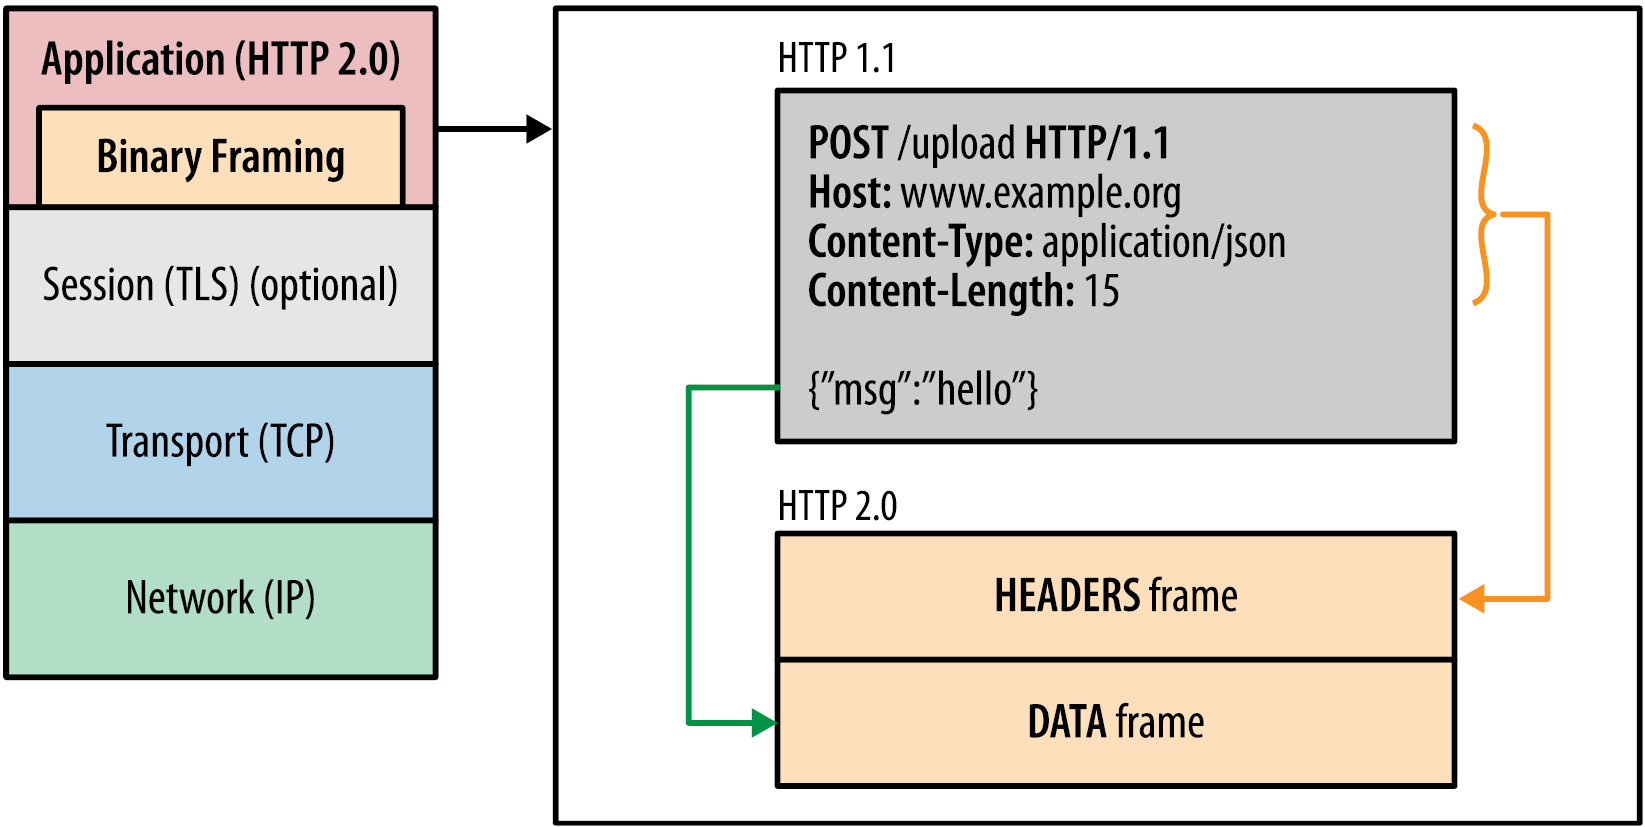
\includegraphics[width=0.75\linewidth]{Images/Binary_framing_layer.png}
	\caption{On the left we can see the binary framing layer inside the application layer and on the right we can see an HTTP/1.1 message being split in two types of frames.}
	\label{fig:binary_framing_layer}
\end{figure}

HTTP/2 introduces a binary framing layer that defines how logical HTTP messages are represented on the connection between a client and a server. This layer is responsible for encapsulating requests, responses, and protocol-control information into a uniform sequence of binary frames. It changes the wire representation of HTTP traffic, but it does not change the semantics of HTTP: methods, status codes, URIs, header fields, and message bodies retain their usual meaning.\\

The framing layer separates the logical structure of an HTTP message from the way that message is transferred. In HTTP/1.x, a request or response is transmitted as a textual message composed of a start line, header fields, an empty line, and an optional body. In HTTP/2, the same logical information is divided into typed frames. Header fields are encoded as compressed header blocks, while message bodies are transferred as data bytes. Other frame types are used for control operations such as prioritization, configuration, flow control, connection testing, and connection shutdown.\\

This design is the basis for the main performance improvements of HTTP/2. Once messages are decomposed into small typed units, frames belonging to different logical exchanges can be interleaved on the same TCP connection and reassembled at the receiving endpoint. The protocol therefore avoids mapping each HTTP exchange to a separate connection and avoids the strict serialization that limited previous HTTP versions.

\section{Streams, Messages, and Frames}

\begin{figure}[!h]
	\centering
	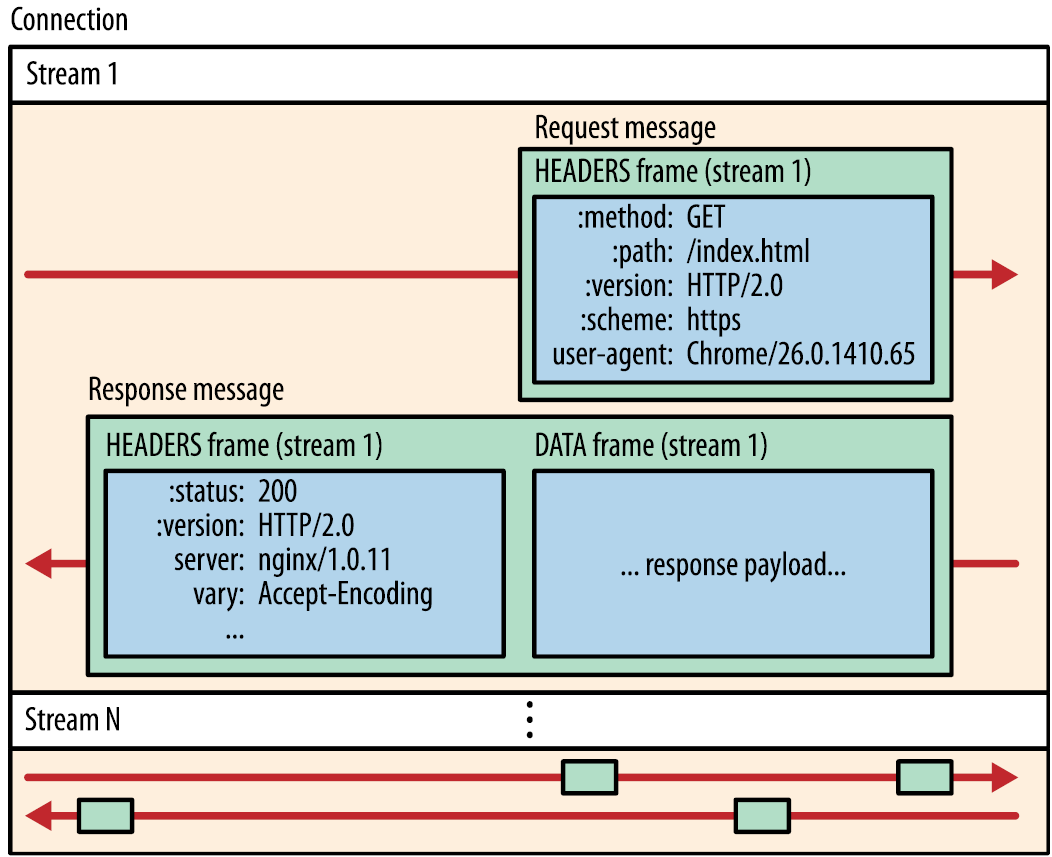
\includegraphics[width=0.6\linewidth]{Images/Streams_messages_frames.png}
	\caption{Example of TCP connection containing streams, messages and frames.}
	\label{fig:streams_messages_frames}
\end{figure}

The framing layer is organized around three concepts: streams, messages, and frames. These concepts form a hierarchy. A connection carries streams, a stream carries messages, and a message is represented by one or more frames (see figure	\ref{fig:streams_messages_frames}).

\subsection{Streams}

A \emph{stream} is a bidirectional flow of bytes within an established HTTP/2 connection. A single TCP connection between a client and a server can carry many streams at the same time. Each stream has a unique identifier, and this identifier is included in the header of each frame that belongs to the stream.\\

A stream is the unit that lets HTTP/2 distinguish independent logical exchanges sharing the same connection. A typical request-response interaction consumes one stream: the client sends a request message on the stream, and the server sends the corresponding response message on the same stream. Since streams are bidirectional, the two endpoints are not limited to a purely one-way transfer pattern. The stream abstraction allows both endpoints to associate all the frames of an exchange without dedicating a separate TCP connection to it.

\subsection{Messages}

A \emph{message} is a complete sequence of frames that maps to one logical HTTP request or response. From the viewpoint of HTTP semantics, a message is still a request or a response. From the viewpoint of the framing layer, it is a structured sequence of one or more frames.\\

A request without a body can be represented by a header block alone. A response with a body is typically represented by header frames followed by data frames. If the header block is too large to fit in a single frame, it can be split into a first header-carrying frame and one or more continuation frames. This decomposition is internal to the protocol: the receiving endpoint reconstructs the logical message before exposing it to the upper HTTP processing logic.

\subsection{Frames}

A \emph{frame} is the smallest unit of communication in HTTP/2. Every frame contains a fixed-format frame header and a payload whose structure depends on the frame type. The frame type determines both the meaning of the payload and the interpretation of the flags carried in the frame header.\\

Frames can carry application data, compressed HTTP header fields, stream-priority information, settings, flow-control updates, server-push promises, and connection-management signals. This uniform frame abstraction makes it possible to interleave heterogeneous information on the same connection while keeping enough metadata to reconstruct streams and messages correctly.\\

Although the physical packets carrying HTTP/2 data may traverse the network through different paths, HTTP/2 operates above TCP and therefore receives an ordered byte stream from the transport layer. The relevant ordering issue at the HTTP/2 layer is that frames belonging to different streams may be interleaved on the same connection. For this reason, each frame carries a numeric stream identifier in its header: the receiver uses this identifier to associate the frame with the correct stream and to reconstruct the corresponding logical HTTP message from the sequence of frames belonging to that stream.

\subsection{Frame Ordering Across the Network Stack}

HTTP/2 frames should not be interpreted as independent datagrams that may be delivered to the HTTP/2 layer in arbitrary order. HTTP/2 is normally carried over TCP, optionally protected by TLS. Therefore, although the physical and network layers may transmit packets through different paths, lose packets, retransmit them, or deliver IP packets out of order, these phenomena are not directly exposed to HTTP/2. TCP hides them by reconstructing the original ordered byte stream before delivering data to the application layer.\\

The layering can be summarized as follows:

\begin{lstlisting}
Physical and IP layers:
packets may be delayed, lost, duplicated, or reordered
	
TCP:
uses sequence numbers, acknowledgments, retransmissions,
and buffering to reconstruct an ordered byte stream
	
HTTP/2:
reads the ordered byte stream and parses it into frames
\end{lstlisting}

Consequently, HTTP/2 frames do not need their own sequence numbers. The byte order seen by the HTTP/2 implementation is already the transmission order reconstructed by TCP. The HTTP/2 receiver parses this ordered byte stream frame by frame. For each frame, the fixed frame header specifies the length of the payload, the frame type, the flags, and the stream identifier. The \texttt{Length} field tells the receiver where the current frame ends; the \texttt{Type} field tells how the payload must be interpreted; the \texttt{Stream Identifier} tells to which logical stream the frame belongs.\\

The stream identifier is therefore not a sequence number. It is a demultiplexing key. It allows the receiver to separate frames belonging to different streams after they have been interleaved on the same TCP connection.\\

For example, the sender may transmit the following ordered sequence of frames:

\begin{lstlisting}
stream 1 HEADERS
stream 3 HEADERS
stream 1 DATA
stream 5 HEADERS
stream 3 DATA
stream 1 DATA END_STREAM
stream 3 DATA END_STREAM
\end{lstlisting}

The receiver observes the same frame order at the HTTP/2 layer, because TCP preserves byte ordering. However, the receiver groups the frames by stream identifier:

\begin{lstlisting}
stream 1:
HEADERS
DATA
DATA END_STREAM

stream 3:
HEADERS
DATA
DATA END_STREAM

stream 5:
HEADERS
\end{lstlisting}

This is the sense in which HTTP/2 supports multiplexing: frames from different streams may be interleaved in the same connection, but they are not delivered to HTTP/2 in a random order. The receiver reconstructs each logical exchange by following the ordered sequence of frames associated with the same stream and the same direction of communication.\\

A separate message identifier is not needed because, in HTTP/2, the stream provides the message context. In the usual client-initiated case, the request is carried by frames sent by the client on a given stream, and the response is carried by frames sent by the server on the same stream. The end of a header block is marked by the \texttt{END\_HEADERS} flag, while the end of the frames sent by one endpoint on that stream is marked by the \texttt{END\_STREAM} flag.\\

For instance, a simple request without a body may be represented as:

\begin{lstlisting}
client -> server:
stream 1 HEADERS END_HEADERS END_STREAM
\end{lstlisting}

The corresponding response may be represented as:

\begin{lstlisting}
server -> client:
stream 1 HEADERS END_HEADERS
stream 1 DATA
stream 1 DATA END_STREAM
\end{lstlisting}

All these response frames belong to the same logical response because they are sent by the server on stream \texttt{1}, in the order delivered by TCP, and because the stream state indicates that they form the response associated with the request on that stream.\\

The only ordering that HTTP/2 explicitly creates at its own layer is the interleaving of frames from different streams. It does not solve arbitrary physical-layer reordering itself. That task belongs to TCP. This distinction is essential: IP packets may be reordered in the network, TCP segments are reassembled into an ordered byte stream, and HTTP/2 frames are parsed from that ordered byte stream and assigned to streams through their stream identifiers.

\subsection{Streams as Message Contexts}

A stream is the logical context in which HTTP/2 carries an HTTP exchange. In the usual client-initiated case, one stream is used for one request and the corresponding response. The client sends the request frames on that stream, and the server sends the response frames on the same stream. A second independent request is not sent later on the same stream; it must use a different stream.\\

For example, a client may request three independent resources by opening three different streams:

\begin{lstlisting}
stream 1:
client request for /page.html
server response with /page.html

stream 3:
client request for /style.css
server response with /style.css

stream 5:
client request for /script.js
server response with /script.js
\end{lstlisting}

The odd stream identifiers in this example indicate streams initiated by the client. The important point is that the stream identifier identifies the exchange context. All frames carrying the request and response for \texttt{/page.html} use stream \texttt{1}; all frames carrying the request and response for \texttt{/style.css} use stream \texttt{3}; and so on.\\

Multiple frames with the same stream identifier do not imply multiple independent messages. They are fragments of the same logical message or of the same logical exchange. A request may require more than one frame because its header block may be split into a \texttt{HEADERS} frame followed by one or more \texttt{CONTINUATION} frames, or because the request has a body carried by \texttt{DATA} frames. Similarly, a response may consist of response headers, zero or more data frames, and optionally trailing headers.\\

A request without a body can be represented as follows:

\begin{lstlisting}
client -> server:
stream 1 HEADERS END_HEADERS END_STREAM
\end{lstlisting}

Here, \texttt{END\_HEADERS} indicates that the header block is complete, while \texttt{END\_STREAM} indicates that the client will not send further frames for its side of stream \texttt{1}. The whole request is contained in a single \texttt{HEADERS} frame.\\

A response with a body can instead be decomposed into several frames:

\begin{lstlisting}
server -> client:
stream 1 HEADERS END_HEADERS
stream 1 DATA
stream 1 DATA
stream 1 DATA END_STREAM
\end{lstlisting}

All these frames belong to the same logical response because they are sent by the server on stream \texttt{1}. The last \texttt{DATA} frame carries the \texttt{END\_STREAM} flag, which indicates that the server has completed its side of the exchange.\\

The stream therefore removes the need for a separate message identifier. The receiver uses the stream identifier to associate each frame with the correct exchange, and it uses the stream state together with flags such as \texttt{END\_HEADERS} and \texttt{END\_STREAM} to determine the boundaries of the header block and of the message body.\\

Server push preserves the same principle, but the exchange is initiated differently. The server does not send the pushed resource on the original client-initiated stream. Instead, it sends a \texttt{PUSH\_PROMISE} frame on the associated stream and reserves a new server-initiated stream for the pushed response. The \texttt{PUSH\_PROMISE} contains request-like header fields describing the resource that the server intends to push.\\

For example:

\begin{lstlisting}
stream 1:
client request for /page.html
server PUSH_PROMISE, promised stream 2 for /script.js
server response with /page.html

stream 2:
server pushed response with /script.js
\end{lstlisting}

In this case, stream \texttt{1} carries the ordinary request-response exchange for \texttt{/page.html}. The promised stream \texttt{2} carries the pushed response for \texttt{/script.js}. The pushed stream does not contain a normal client request sent by the client; the request context is represented by the \texttt{PUSH\_PROMISE} sent on the associated stream.\\

Thus, a stream should be understood as the unit that binds frames to a specific HTTP exchange. Frames may be numerous and interleaved with frames from other streams, but they do not create a sequence of independent messages on the same stream. A new independent resource exchange requires a new stream.

\section{Multiplexing over a Single Connection}

\begin{figure}[!h]
	\centering
	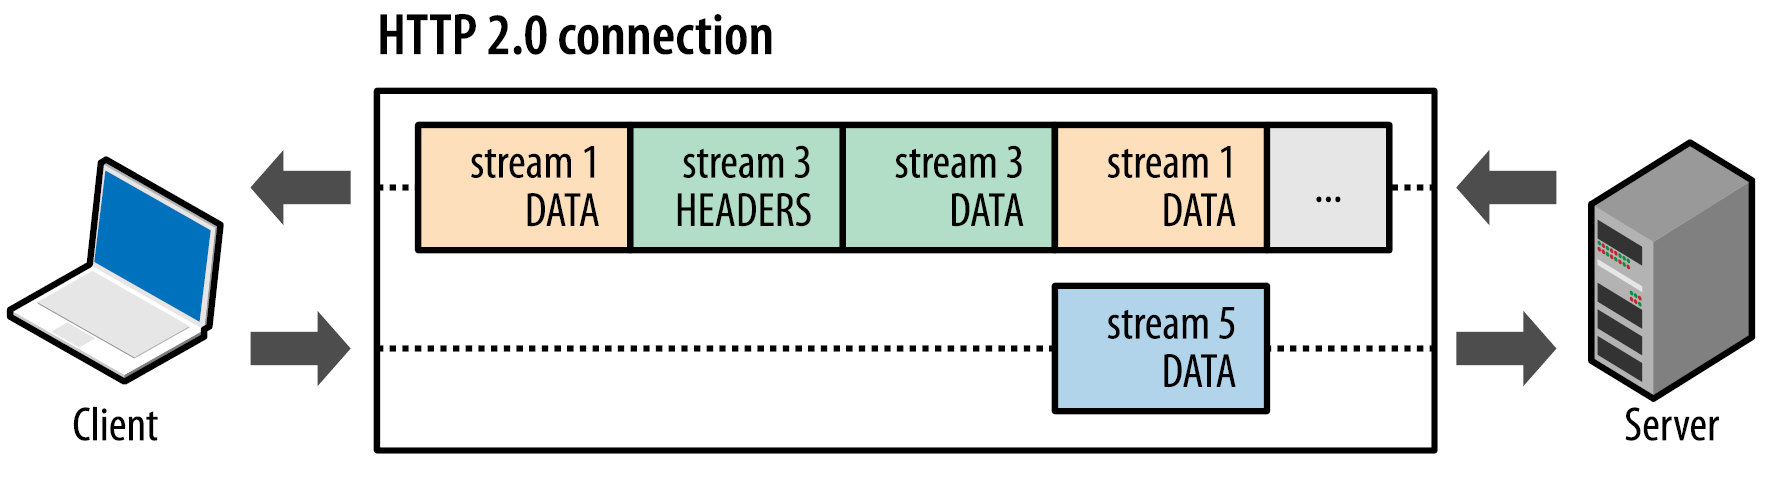
\includegraphics[width=\linewidth]{Images/Multiplexing.png}
	\caption{Example of HTTP 2.0 connection with multiplexing. In this example the client is transmitting a DATA frame (stream 5) to the server and the server is transmitting an interleaved sequence of frames to the client for streams 1 and 3. As a result, there are three parallel streams in flight.}
	\label{fig:multiplexing}
\end{figure}

HTTP/1.0 allowed only one request-response exchange per TCP connection. HTTP/1.1 improved this model with persistent connections and request pipelining, but pipelining was only a partial solution: outstanding requests could be sent before previous responses were received, yet the response ordering constraints and practical deployment limitations still made the model prone to blocking and inefficient use of available capacity.\\

HTTP/2 replaces this model with full request and response multiplexing. All communication between a client and a server can occur over a single TCP connection that carries multiple bidirectional streams. The frames belonging to these streams are serialized onto the same connection, but they need not be grouped by message or by stream. A frame from one response can be followed by a frame from another response, then by a frame from a client request body, and then by another frame from the first response.\\

The stream identifier in each frame header makes this interleaving unambiguous. The receiver reads the byte stream delivered by TCP, observes the frame boundaries, inspects the stream identifier of each frame, and appends the frame payload to the corresponding logical stream. In this way, HTTP/2 can carry multiple independent exchanges concurrently while preserving the logical separation required by HTTP semantics.

\subsection{Interleaved Requests and Responses}

Multiplexing applies in both directions. A client can have several outstanding requests without opening several TCP connections, and a server can send several responses in parallel without waiting for one response to complete before starting another. For example, while a client is sending a \texttt{DATA} frame on stream 5, the server may send an interleaved sequence of frames for streams 1 and 3 on the same connection. At that moment, three streams are active concurrently: one carrying data from the client to the server, and two carrying server-to-client response information (see figure \ref{fig:multiplexing}).\\

This behavior is the core difference between HTTP/2 multiplexing and HTTP/1.1 persistent connections. Persistence reuses a connection across several exchanges; multiplexing allows several exchanges to make progress during the same period of time on that connection.

\subsection{Reassembly}

Reassembly is based on frame metadata rather than on separate transport connections. The receiver does not infer message boundaries from TCP connections. Instead, it uses the frame type, flags, payload length, and stream identifier to determine how each frame contributes to a stream and when a logical message has ended.\\

This mechanism also allows frames from different streams to be interleaved without ambiguity. The sequence seen on the wire is a connection-level sequence of frames; the sequence reconstructed by the endpoint is a set of stream-local sequences. HTTP/2 therefore separates the ordering of bytes on the connection from the logical organization of HTTP requests and responses.

\section{Performance Consequences of Multiplexing}

The ability to break an HTTP message into independent frames, interleave those frames with frames from other streams, and reassemble them at the other endpoint is the central enhancement introduced by HTTP/2. It changes how the protocol uses the underlying TCP connection and how web resources are scheduled.\\

A first consequence is that multiple requests can be in flight without blocking on a single request. The client does not need to wait for the completion of one exchange before progressing with another. A second consequence is that multiple responses can be interleaved. If a large response is being transferred, the server can still send frames belonging to a smaller or more important response instead of forcing the latter to wait until the large response has completed.\\

A third consequence is better connection utilization. A single connection can carry many logical exchanges, reducing the need for multiple TCP connections to the same server. This reduces connection-management overhead and gives the protocol a single place where it can coordinate multiplexing, prioritization, and flow control.

\subsection{Application-Layer Blocking}

HTTP/2 multiplexing addresses application-layer head-of-line blocking caused by serial request-response processing. In HTTP/1.x, a slow or large resource could delay subsequent resources when exchanges were forced into a sequential pattern. HTTP/2 avoids this specific limitation by allowing frames from other streams to make progress while one stream is still active.\\

This improvement should not be confused with eliminating all forms of blocking. HTTP/2 commonly runs over TCP, and TCP still provides an ordered byte stream. If packet loss occurs, TCP may delay delivery of later bytes until missing bytes have been retransmitted. HTTP/2 removes the protocol-level serialization of HTTP messages, but it does not remove transport-layer effects imposed by TCP.

\subsection{Reduced Need for HTTP/1.x Workarounds}

\begin{figure}
	\centering
	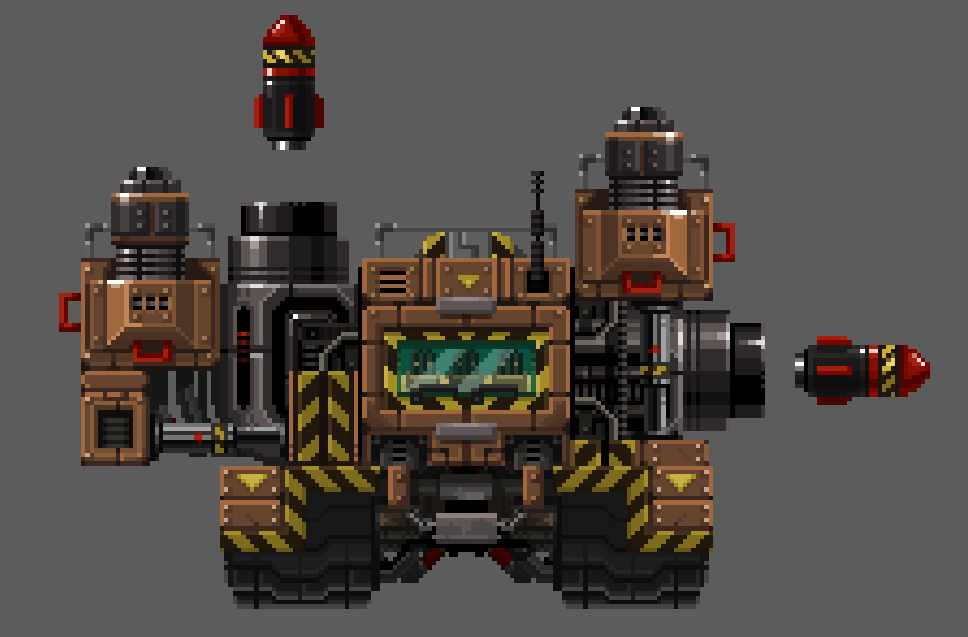
\includegraphics[width=\linewidth]{Images/Image_sprite.jpg}
	\caption{Tank and rocket sprites from Broforce}
	\label{fig:image_sprite}
\end{figure}

\begin{figure}
	\centering
	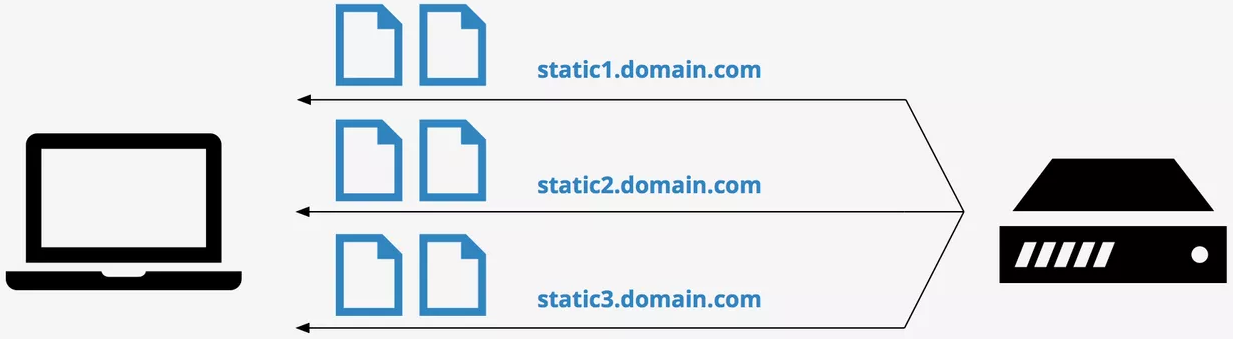
\includegraphics[width=\linewidth]{Images/Domain_sharding.png}
	\caption{Domain sharding in HTTP/1.x. Static resources are distributed across multiple hostnames, such as \texttt{static1.domain.com}, \texttt{static2.domain.com}, and \texttt{static3.domain.com}, so that the browser can open more parallel TCP connections to the same logical service. This workaround reduces request queuing caused by per-host connection limits, but increases connection-management overhead and becomes largely unnecessary with HTTP/2 multiplexing.}
	\label{fig:domain_sharding}
\end{figure}

Before HTTP/2, web applications often compensated for the limitations of HTTP/1.x using techniques that reduced the number of requests or increased the number of parallel connections. Common examples include resource concatenation, image sprites, and domain sharding.\\

Resource concatenation combines multiple small files, such as scripts or style sheets, into a single larger file. This reduces request overhead in HTTP/1.x, but it also reduces cache granularity: a small change in one component can force the client to re-fetch a larger bundle. Image sprites apply a similar idea to images, combining many small images into a single image file and selecting the visible region at the application layer, often through CSS (see figure \ref{fig:image_sprite}). Domain sharding uses multiple hostnames to bypass per-host connection limits and force the browser to open more TCP connections, but it also increases connection setup overhead and weakens the benefits of centralized scheduling (see figure \ref{fig:domain_sharding}).\\

HTTP/2 targets the protocol limitation that made these workarounds attractive. Since many resources can be requested and transferred concurrently over a single connection, the protocol no longer requires applications to artificially reduce request counts or split traffic across hostnames merely to obtain concurrency. In practice, decisions about bundling, caching, and hostnames still depend on deployment details, network conditions, and implementation behavior. The architectural reason for those workarounds, however, is substantially reduced by the HTTP/2 framing and multiplexing model.

\chapter{HTTP/2 Frames, Stream Control, and Prioritization}

\section{Frame Format}

\begin{figure}[!h]
	\centering
	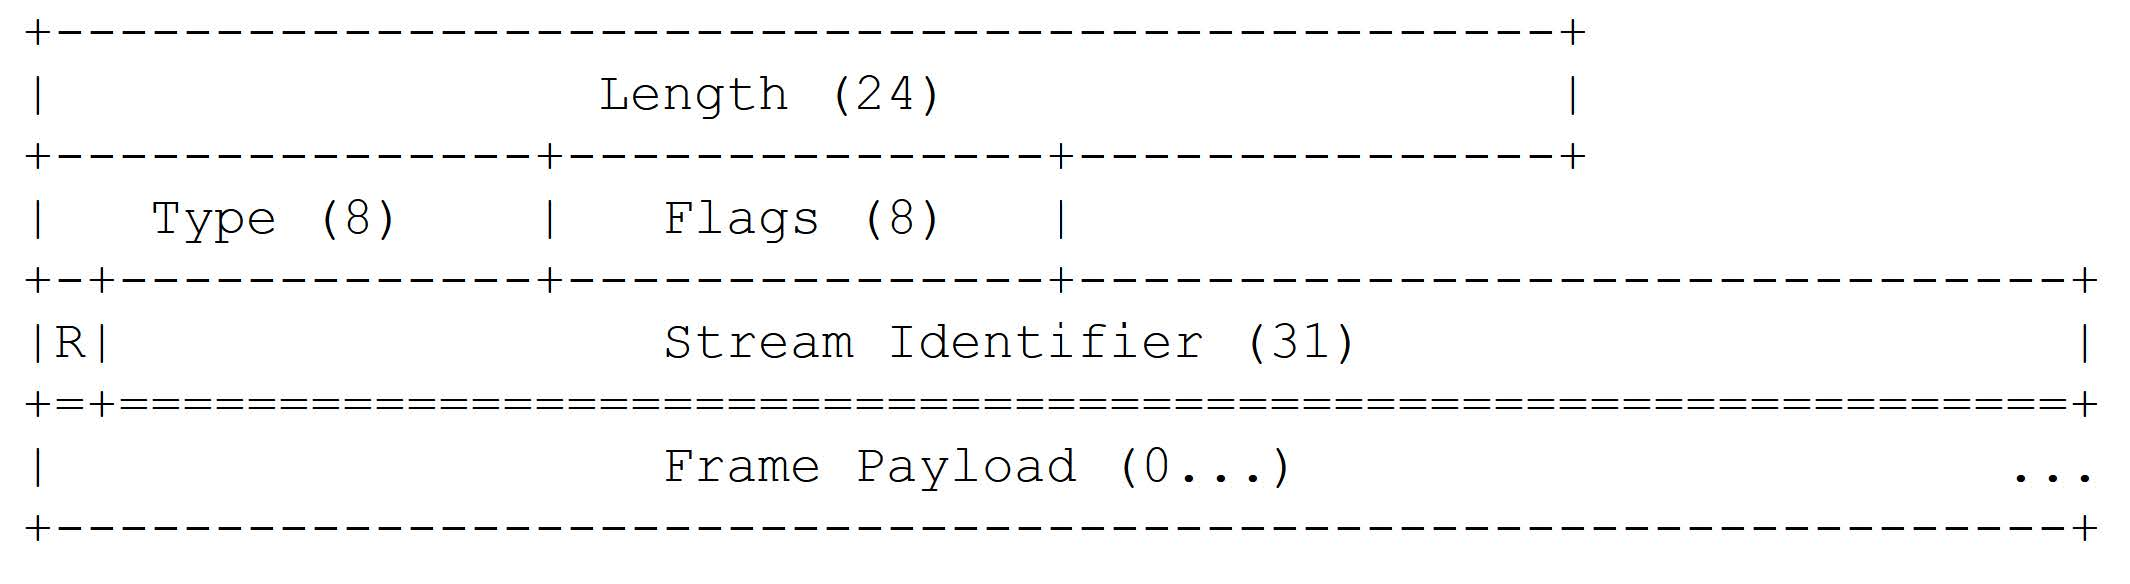
\includegraphics[width=\linewidth]{Images/Frame_format.jpg}
	\caption{HTTP/2 frame format}
	\label{fig:frame_format}
\end{figure}

All HTTP/2 frames share a common frame header followed by a payload. The frame header identifies the size and meaning of the payload, the stream to which the frame belongs, and a small set of frame-specific Boolean properties.\\

The frame header contains the following fields:

\begin{center}
	\begin{tabularx}{\linewidth}{llX}
		\hline
		
		\textbf{Field} & \textbf{Size} & \textbf{Meaning} \\
		\hline
		
		Length & 24 bits & The size, in bytes, of the frame payload, excluding the fixed 9-byte frame header. Since it is encoded on 24 bits, its theoretical range is from 0 to $2^{24}-1$ bytes. However, the maximum payload size accepted on a connection is limited by \texttt{SETTINGS\_MAX\_FRAME\_SIZE}, whose default value is $2^{14}=16{,}384$ bytes and whose maximum allowed value is $2^{24}-1$ bytes. \\ \hline
		
		Type & 8 bits & Frame type, which determines payload format and semantics \\ \hline
		
		Flags & 8 bits & Frame-specific Boolean flags \\ \hline
		
		R & 1 bit & Reserved bit, currently set to zero \\ \hline
		
		Stream identifier & 31 bits & Identifier of the stream to which the frame belongs \\ \hline
		
		Payload & Variable & Type-specific data \\ \hline
	\end{tabularx}
\end{center}

The payload length refers only to the frame payload, not to the frame header. All fields before the payload constitute the frame header. A stream identifier equal to zero is reserved for frames that refer to the entire connection rather than to a specific stream. This distinction is essential because HTTP/2 contains both stream-level operations, such as data transfer for a particular request or response, and connection-level operations, such as settings negotiation.\\

The flags field is intentionally generic. Its meaning depends on the frame type. For instance, a flag may indicate the end of a stream for one frame type, the end of a header block for another frame type, or the presence of optional padding. This design keeps the common frame header compact while allowing each frame type to define the control bits it needs.

\section{Frame Types}

HTTP/2 defines a small set of frame types. Some frame types carry the content of logical HTTP messages, while others regulate the behavior of streams and of the connection.

\begin{center}
	\begin{tabular}{lcl}
		\hline
		Frame type & Type code & Main role \\
		\hline
		\texttt{DATA} & 0 & Carries message-body bytes associated with a stream \\
		\texttt{HEADERS} & 1 & Carries compressed HTTP header fields \\
		\texttt{PRIORITY} & 2 & Communicates stream priority information \\
		\texttt{RST\_STREAM} & 3 & Terminates a stream immediately \\
		\texttt{SETTINGS} & 4 & Negotiates connection configuration parameters \\
		\texttt{PUSH\_PROMISE} & 5 & Announces a server-initiated stream for a pushed resource \\
		\texttt{PING} & 6 & Tests connection liveness and estimates round-trip time \\
		\texttt{GOAWAY} & 7 & Initiates graceful connection shutdown \\
		\texttt{WINDOW\_UPDATE} & 8 & Updates the flow-control window \\
		\texttt{CONTINUATION} & 9 & Continues a header block split across frames \\
		\hline
	\end{tabular}
\end{center}

The distinction between content-carrying frames and control frames is important. \texttt{DATA} and \texttt{HEADERS} frames directly represent parts of logical HTTP messages. Other frames modify how streams are scheduled, how much data can be sent, which resources may be pushed, or how a connection is configured and closed. Because these operations share the same framing format, they can coexist on the same connection and be processed according to their scope: stream-specific or connection-wide.

\section{DATA Frames}

A \texttt{DATA} frame transports arbitrary variable-length byte sequences associated with a stream. It is the frame type used for the body of HTTP requests and responses. A request with an entity body or a response containing an HTML document, image, script, style sheet, or other payload uses \texttt{DATA} frames for the body bytes.

\subsection{Flags}

A \texttt{DATA} frame defines two flags:

\begin{itemize}
    \item \texttt{END\_STREAM} (\texttt{0x1}): when set, it indicates that this frame is the last frame that the endpoint will send for the stream.
    \item \texttt{PADDED} (\texttt{0x8}): when set, it indicates that the payload includes a pad-length field and padding bytes.
\end{itemize}

The \texttt{END\_STREAM} flag is part of the stream-closing logic. A frame without this flag does not terminate the sending direction of the stream. A frame with this flag states that the sender has no further frames to transmit on that stream.

\subsection{Payload Structure}

\begin{figure}[!h]
	\centering
	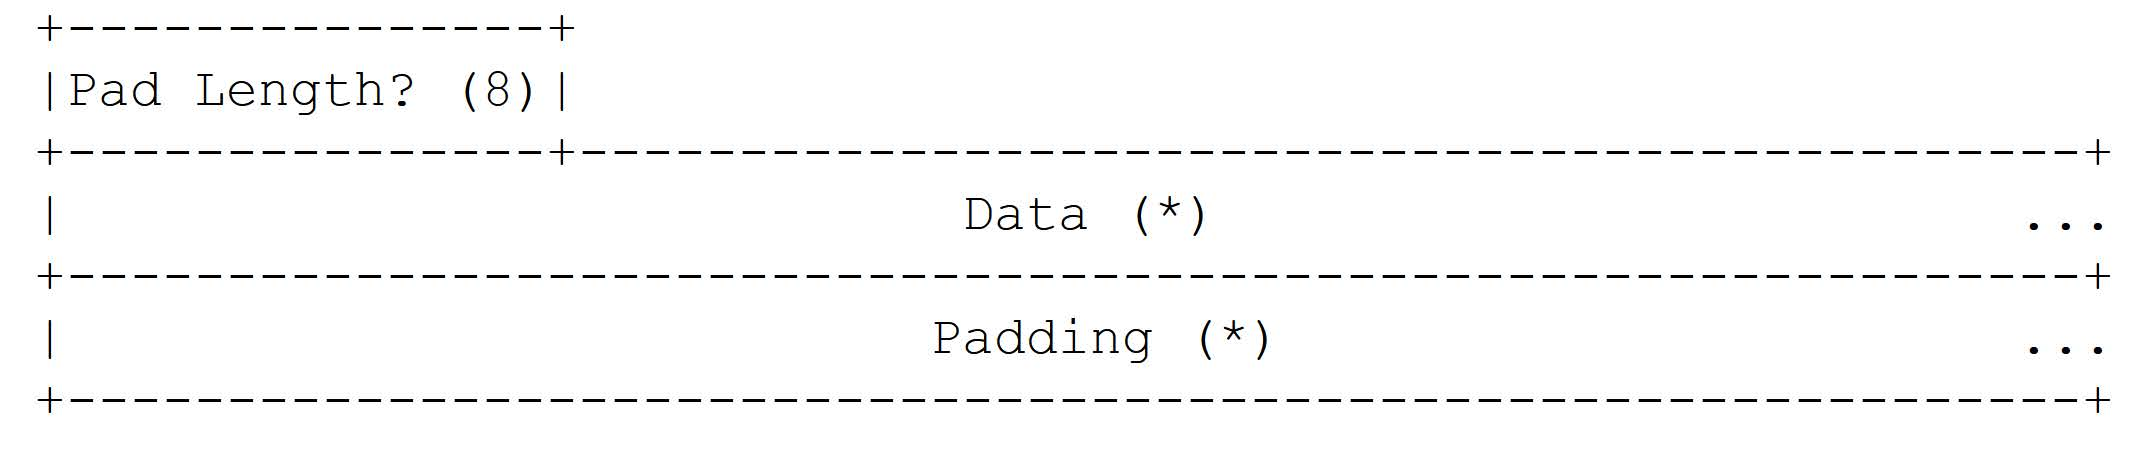
\includegraphics[width=\linewidth]{Images/Data_frame_payload.jpg}
	\caption{Data frame payload structure}
	\label{fig:data_frame_payload}
\end{figure}

The payload of a \texttt{DATA} frame may contain the following fields:

\begin{itemize}
    \item \texttt{Pad Length}, present only when \texttt{PADDED} is set, specifies the length of the padding field in bytes.
    \item \texttt{Data} contains the actual message-body bytes.
    \item \texttt{Padding}, present only when \texttt{PADDED} is set, contains bytes that are not part of the application payload.
\end{itemize}

Padding can be used to obscure the exact size of the transmitted message. The receiver knows the total frame payload length from the frame header and, when padding is present, knows the padding length from the \texttt{Pad Length} field. It can therefore determine the size of the useful data by subtracting the padding information from the total payload length. Padding does not change the HTTP semantics of the message; it only changes the wire representation.

\section{HEADERS Frames}

A \texttt{HEADERS} frame carries a compressed HTTP header block fragment. Header fields that would appear textually in an HTTP/1.x message are encoded by the HTTP/2 header-compression mechanism and transported as binary data inside one or more header-carrying frames.\\

A request without a body can be represented by a \texttt{HEADERS} frame with \texttt{END\_STREAM} set. A response with a body normally starts with a \texttt{HEADERS} frame containing the response header fields, followed by one or more \texttt{DATA} frames containing the response body.

\subsection{Flags}

A \texttt{HEADERS} frame defines four flags:

\begin{itemize}
    \item \texttt{END\_STREAM} (\texttt{0x1}): when set, it indicates that the frame is the last one the endpoint will send for the stream.
    \item \texttt{END\_HEADERS} (\texttt{0x4}): when set, it indicates that the frame contains the complete header block and is not followed by \texttt{CONTINUATION} frames for the same header block.
    \item \texttt{PADDED} (\texttt{0x8}): when set, it indicates that the payload includes a pad-length field and padding.
    \item \texttt{PRIORITY} (\texttt{0x20}): when set, it indicates that the payload includes the stream-priority fields.
\end{itemize}

The distinction between \texttt{END\_STREAM} and \texttt{END\_HEADERS} is essential. The former concerns the lifetime of the stream in the sending direction; the latter concerns only the end of the current header block. A message may finish its header block and still continue with data frames. Conversely, a message with no body can finish both the header block and the stream in the same \texttt{HEADERS} frame.

\subsection{Payload Structure}

\begin{figure}[!h]
	\centering
	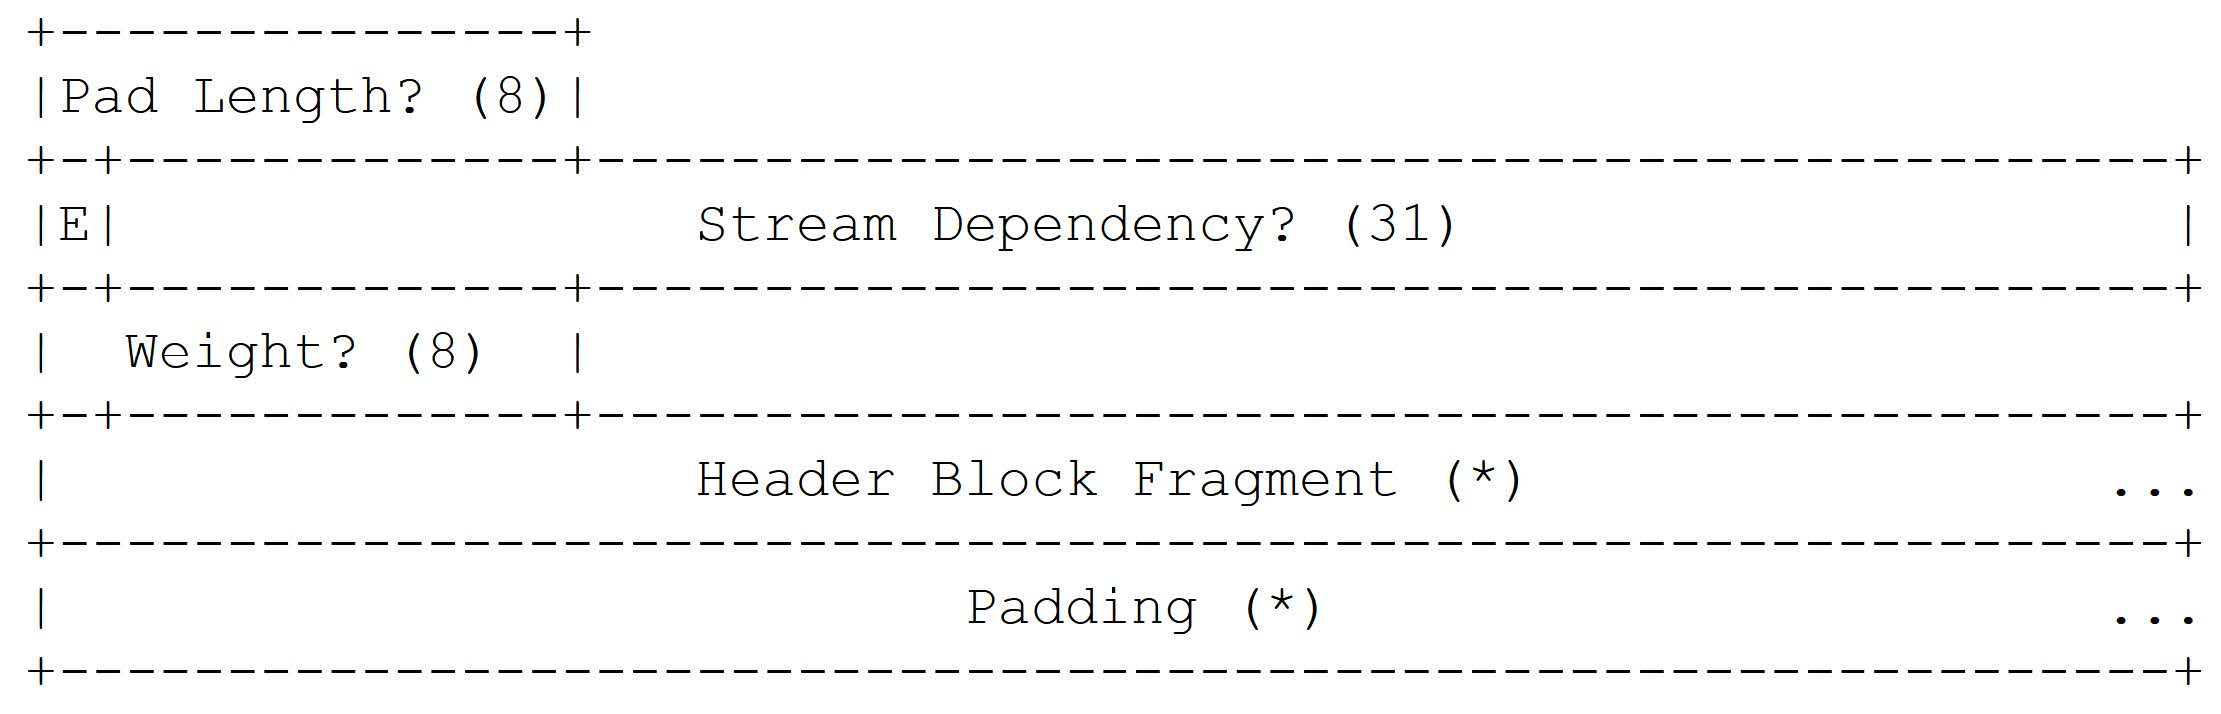
\includegraphics[width=\linewidth]{Images/Header_frame_payload.jpg}
	\caption{Header frame payload structure}
	\label{fig:header_frame_payload}
\end{figure}

The payload of a \texttt{HEADERS} frame may contain the following fields:

\begin{itemize}
    \item \texttt{Pad Length}, present only when \texttt{PADDED} is set.
    \item \texttt{E}, \texttt{Stream Dependency}, and \texttt{Weight}, present only when \texttt{PRIORITY} is set.
    \item \texttt{Header Block Fragment}, containing a fragment of the compressed header block.
    \item \texttt{Padding}, present only when \texttt{PADDED} is set.
\end{itemize}

The priority fields allow priority information to be transmitted together with the headers that create or describe a stream. The header block fragment is the part that corresponds to the HTTP header fields themselves after compression. If the complete header block does not fit in a single \texttt{HEADERS} frame, the block is continued using \texttt{CONTINUATION} frames.

\newpage
\section{CONTINUATION Frames}

\begin{figure}[!h]
	\centering
	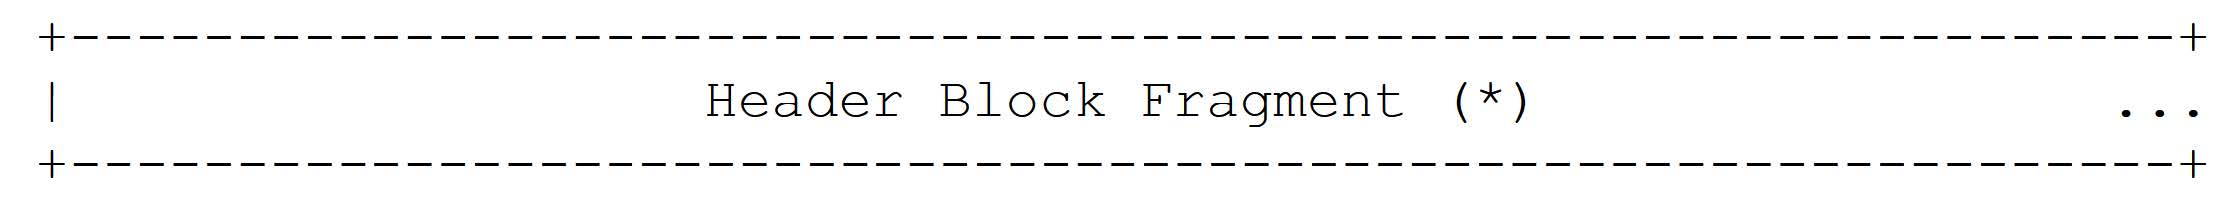
\includegraphics[width=\linewidth]{Images/Continuation_frame_payload.jpg}
	\caption{Continuation frame payload structure}
	\label{fig:continuation_frame_payload}
\end{figure}

A \texttt{CONTINUATION} frame extends a header block that began in a \texttt{HEADERS} frame or in a \texttt{PUSH\_PROMISE} frame. Its payload consists of another header block fragment belonging to the same stream and to the same logical header block (see figure \ref{fig:continuation_frame_payload}).\\

The need for this frame type follows from the separation between message semantics and frame boundaries. An HTTP header block is a logical object, while an HTTP/2 frame is a bounded transport unit. When a header block is too large for one frame, the protocol does not change the meaning of the headers; it only splits their binary representation across a sequence of frames.\\

Continuation is therefore not a separate HTTP message. It is a continuation of the same compressed header block. The receiver reconstructs the complete header block by concatenating the fragments in the correct sequence and then decompressing and interpreting the resulting block as HTTP header fields.

\section{Stream Identifiers and Stream Use}

Streams can be initiated by either endpoint. Client-initiated streams use odd-numbered identifiers in increasing order; server-initiated streams use even-numbered identifiers in increasing order. The identifier makes it possible to distinguish logical exchanges that are multiplexed over the same TCP connection.\\

Stream identifiers cannot be reused. After a stream has been closed, its identifier is consumed permanently for that connection. If the identifier space is exhausted, the current connection must be closed and a new connection must be opened. This rule avoids ambiguity: a frame carrying a given stream identifier can only belong to one stream during the lifetime of the connection.\\

A stream can be closed by either endpoint. In the common request-response pattern, one HTTP request and its corresponding HTTP response fully consume a single stream. Other streams can be active at the same time, and their frames can be interleaved on the connection. The receiver processes frames in the order in which they are received on the connection and uses the stream identifier to dispatch each frame to the correct stream state.

\newpage
\section{Stream Priority}

\begin{figure}[!h]
	\centering
	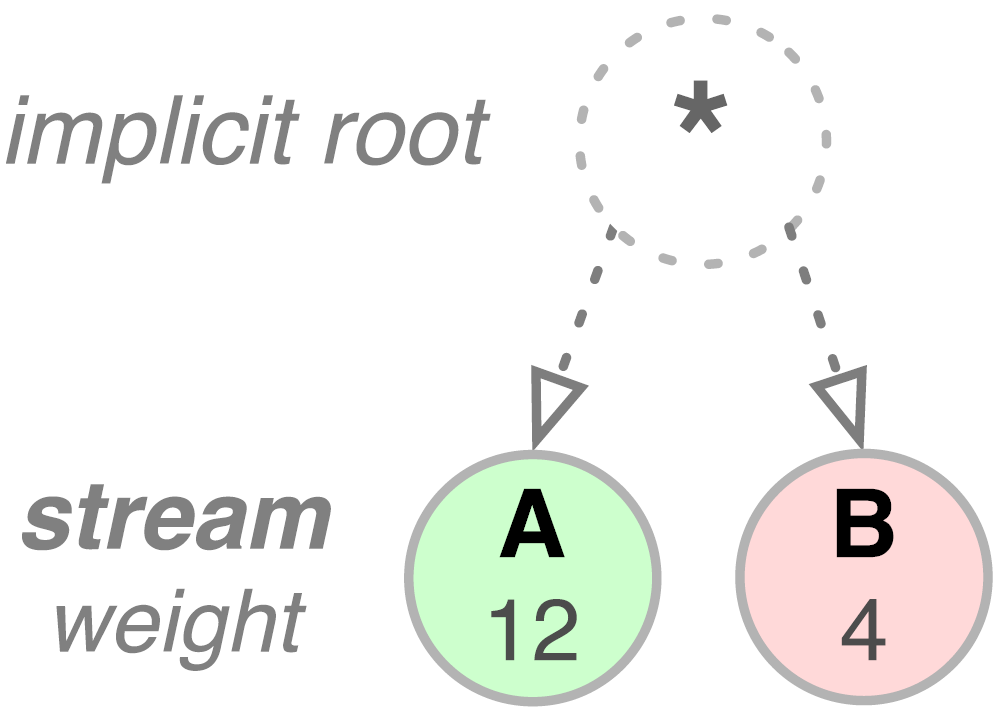
\includegraphics[width=0.5\linewidth]{Images/Prioritization_tree_explanation.png}
	\caption{Basic prioritization tree with labeled nodes. -- The priority tree has an implicit root node, which represents the whole connection rather than a real HTTP/2 stream. Streams that do not depend on another stream are attached to this root, identified at the protocol level by dependency on stream \texttt{0}. The root has no weight and carries no data; it only provides the top-level scheduling context. If several streams are direct children of the root, the resources available at the connection level are divided among them proportionally to their weights.}
	\label{fig:prioritization_tree_explanation}
\end{figure}

HTTP/2 includes a priority mechanism that lets a client express which streams should receive preferential treatment. This is necessary because multiplexing creates a scheduling problem: when several streams are active at the same time, the server must decide how to allocate transmission opportunities and other resources among them.\\

Each stream can be associated with:

\begin{itemize}
    \item an integer weight between 1 and 256;
    \item an explicit dependency on another stream.
\end{itemize}

Dependencies and weights form a prioritization tree. A dependency states that one stream is the parent of another. The intended scheduling model is that parent streams should be processed before their children. Weights then divide resources among sibling streams. If several streams share the same parent, each sibling receives a share proportional to its weight:

\[
\text{share}_i = \frac{w_i}{\sum_{j=1}^{n} w_j}
\]

where \(w_i\) is the weight of stream \(i\) and the denominator is the sum of the weights of all sibling streams under the same parent.\\

For example, if two sibling streams have weights 12 and 4, their total weight is 16. The first stream expresses a preferred share of \(12/16 = 3/4\), while the second expresses a preferred share of \(4/16 = 1/4\). The protocol does not define the exact resource to which this proportion must be applied. A server can use the priority information to guide bandwidth allocation, CPU scheduling, memory usage, or internal queuing decisions.\\

Priority information can be sent in a \texttt{HEADERS} frame or in a dedicated \texttt{PRIORITY} frame. In both cases, priority is a preference rather than a strict requirement. The server is allowed to use the information to optimize transfer order, but the protocol does not force a specific scheduling algorithm.

\subsection{Priority Tree Example: Dependencies, Weights, and Scheduling}

\begin{figure}[!h]
	\centering
	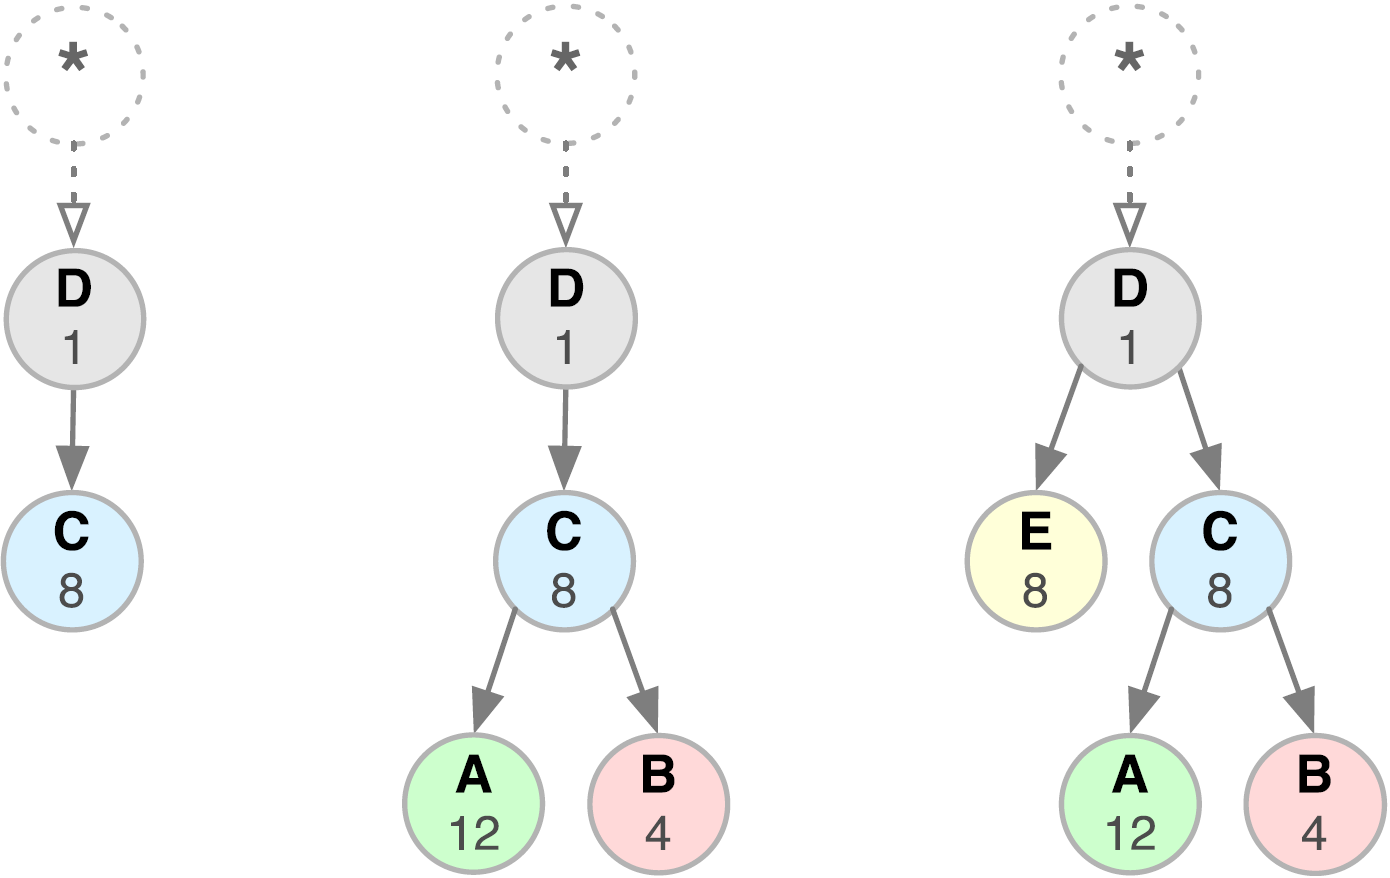
\includegraphics[width=0.5\linewidth]{Images/Prioritization_tree_example.png}
	\caption{Prioritization tree example}
	\label{fig:http2-priority-tree-example}
\end{figure}

Consider the priority tree in Figure~\ref{fig:http2-priority-tree-example}. The dashed node at the top represents the implicit root of the HTTP/2 priority tree. It is not a real stream; it is a virtual scheduling node that represents the whole connection. Streams that do not depend on another real stream are attached to this implicit root.\\

The final tree represented by the example can be written as follows:

\begin{lstlisting}
implicit root
	└── D   weight 1
	    ├── E   weight 8
	    └── C   weight 8
	        ├── A   weight 12
	        └── B   weight 4
\end{lstlisting}

The number inside each node is the stream weight. A stream dependency expresses a scheduling preference: a parent stream should be served before the streams that depend on it, unless the parent stream is closed or cannot currently make progress. The weight expresses how the available resources are divided among sibling streams, that is, among streams that have the same parent.\\

This means that the priority tree should not be read as a depth-first traversal. HTTP/2 prioritization is not an algorithm that visits one node, expands one child completely, and then moves to the next child. Instead, it is a recursive weighted scheduling model. At each level of the tree, the resources available to a parent are divided among its eligible children proportionally to their weights.

\subsubsection{Why the picture can be misleading}

The sequence of drawings in the example may suggest that stream \texttt{C} is expanded first, then its children \texttt{A} and \texttt{B} are processed, and only afterwards stream \texttt{E} is considered. This interpretation would resemble a depth-first search:

\begin{lstlisting}
	D, C, A, B, E
\end{lstlisting}

This is not the intended meaning of the priority tree.\\

The drawings are better interpreted as successive configurations of the priority tree, or as an illustrative construction of the tree. The fact that \texttt{A} and \texttt{B} are shown before \texttt{E} in the sequence does not imply that \texttt{A} and \texttt{B} are scheduled before \texttt{E}. Once the final tree exists, \texttt{E} and \texttt{C} are siblings because they both depend directly on \texttt{D}. Therefore, they must be considered at the same dependency level.\\

The misleading aspect of the picture is that the graphical order of appearance can be confused with a processing order. The actual scheduling order is determined by dependencies and weights, not by the order in which nodes are drawn.

\subsubsection{Parent-Before-Child Preference}

The dependency relation gives priority to a parent over its descendants. In the example, \texttt{D} is the only direct child of the implicit root. Therefore, the whole connection-level capacity is assigned first to the branch rooted at \texttt{D}.\\

Let \(R\) be the total scheduling capacity available at the implicit root. Since \texttt{D} is the only child of the root, its share is

\[
\operatorname{share}(D)
=
\frac{1}{1}R
=
R.
\]

If stream \texttt{D} has data to send and can make progress, it is preferred over its children. In that case, the effective allocation is

\[
\operatorname{share}(D)=R,
\qquad
\operatorname{share}(C)=0,
\qquad
\operatorname{share}(E)=0,
\qquad
\operatorname{share}(A)=0,
\qquad
\operatorname{share}(B)=0.
\]

The children of \texttt{D} become relevant only when \texttt{D} is closed, has no data ready, or is otherwise unable to use the available capacity.

\subsubsection{Scheduling the Children of \texttt{D}}

Once \texttt{D} cannot use its allocation, the scheduler considers its children. In the final tree, \texttt{D} has two children:

\begin{itemize}
	\item stream \texttt{C}, with weight \(8\);
	\item stream \texttt{E}, with weight \(8\).
\end{itemize}

The resources available below \texttt{D} are divided among \texttt{C} and \texttt{E} proportionally to their weights. Since the two weights are equal, the two branches receive the same share:

\[
\operatorname{share}(C)
=
\frac{8}{8+8}R
=
\frac{1}{2}R,
\]

\[
\operatorname{share}(E)
=
\frac{8}{8+8}R
=
\frac{1}{2}R.
\]

At this level, \texttt{C} and \texttt{E} are peers. The scheduler should not process the whole subtree of \texttt{C} before considering \texttt{E}. Instead, the branch rooted at \texttt{C} and the stream \texttt{E} share the available capacity equally.\\

If both \texttt{C} and \texttt{E} have data ready and can make progress, then the effective allocation is

\[
\operatorname{share}(C)=\frac{1}{2}R,
\qquad
\operatorname{share}(E)=\frac{1}{2}R,
\qquad
\operatorname{share}(A)=0,
\qquad
\operatorname{share}(B)=0.
\]

Streams \texttt{A} and \texttt{B} do not receive capacity in this case, because they depend on \texttt{C}. They become eligible only when \texttt{C} itself is closed or cannot currently make progress.

\subsubsection{Scheduling the Children of \texttt{C}}

Stream \texttt{C} has two children:

\begin{itemize}
	\item stream \texttt{A}, with weight \(12\);
	\item stream \texttt{B}, with weight \(4\).
\end{itemize}

These children share only the capacity assigned to the \texttt{C} branch. They do not compete directly with \texttt{E} for the whole capacity \(R\). Since \texttt{C} receives one half of the capacity below \texttt{D}, the maximum capacity available to the subtree of \texttt{C} is

\[
\operatorname{share}(C\text{-branch})
=
\frac{1}{2}R.
\]

Within this branch, \texttt{A} and \texttt{B} divide the capacity proportionally to their weights:

\[
\operatorname{relative\_share}(A \mid C)
=
\frac{12}{12+4}
=
\frac{12}{16}
=
\frac{3}{4},
\]

\[
\operatorname{relative\_share}(B \mid C)
=
\frac{4}{12+4}
=
\frac{4}{16}
=
\frac{1}{4}.
\]

Therefore, if \texttt{D} and \texttt{C} cannot make progress, while \texttt{E}, \texttt{A}, and \texttt{B} can make progress, the effective connection-level shares are

\[
\operatorname{share}(E)
=
\frac{1}{2}R,
\]

\[
\operatorname{share}(A)
=
\frac{1}{2}R \cdot \frac{3}{4}
=
\frac{3}{8}R,
\]

\[
\operatorname{share}(B)
=
\frac{1}{2}R \cdot \frac{1}{4}
=
\frac{1}{8}R.
\]

The complete allocation in this case is therefore

\[
\operatorname{share}(E)
:
\operatorname{share}(A)
:
\operatorname{share}(B)
=
\frac{1}{2}
:
\frac{3}{8}
:
\frac{1}{8}.
\]

Equivalently, using a common denominator:

\[
\operatorname{share}(E)
:
\operatorname{share}(A)
:
\operatorname{share}(B)
=
4
:
3
:
1.
\]

This result shows why the tree is not depth-first. If the scheduling were depth-first, one might expect \texttt{A} and \texttt{B} to be processed before \texttt{E}, because they appear under \texttt{C} in the intermediate drawing. In the actual HTTP/2 priority model, \texttt{E} receives one half of the available capacity because it is a sibling of \texttt{C}. The children of \texttt{C} receive only subdivisions of \texttt{C}'s half.

\subsubsection{Summary of the Possible Scheduling Cases}

The effective allocation depends on which streams are able to use their assigned capacity. The following cases summarize the example.\\

If \texttt{D} is active and can make progress, it receives the full capacity:

\[
\operatorname{share}(D)=R.
\]

If \texttt{D} cannot make progress, but both \texttt{C} and \texttt{E} can make progress, then \texttt{C} and \texttt{E} split the capacity equally:

\[
\operatorname{share}(C)=\frac{1}{2}R,
\qquad
\operatorname{share}(E)=\frac{1}{2}R.
\]

If \texttt{D} and \texttt{C} cannot make progress, but \texttt{E}, \texttt{A}, and \texttt{B} can make progress, then the allocation becomes:

\[
\operatorname{share}(E)=\frac{1}{2}R,
\qquad
\operatorname{share}(A)=\frac{3}{8}R,
\qquad
\operatorname{share}(B)=\frac{1}{8}R.
\]

Thus, the final tree expresses the following preference structure:

\begin{itemize}
	\item \texttt{D} is preferred before everything below it.
	\item If \texttt{D} cannot use the capacity, its children \texttt{C} and \texttt{E} share the capacity equally.
	\item The branch rooted at \texttt{C} receives only the share assigned to \texttt{C}.
	\item If \texttt{C} cannot use that share directly, its children \texttt{A} and \texttt{B} divide it according to weights \(12\) and \(4\).
	\item \texttt{A} and \texttt{B} do not have priority over \texttt{E}; they are descendants of \texttt{C}, while \texttt{E} is a sibling of \texttt{C}.
\end{itemize}

The priority tree is therefore a recursive weighted scheduling structure. It is not a strict traversal order and it is not equivalent to depth-first search.

\section{PRIORITY Frames}

\begin{figure}[!h]
	\centering
	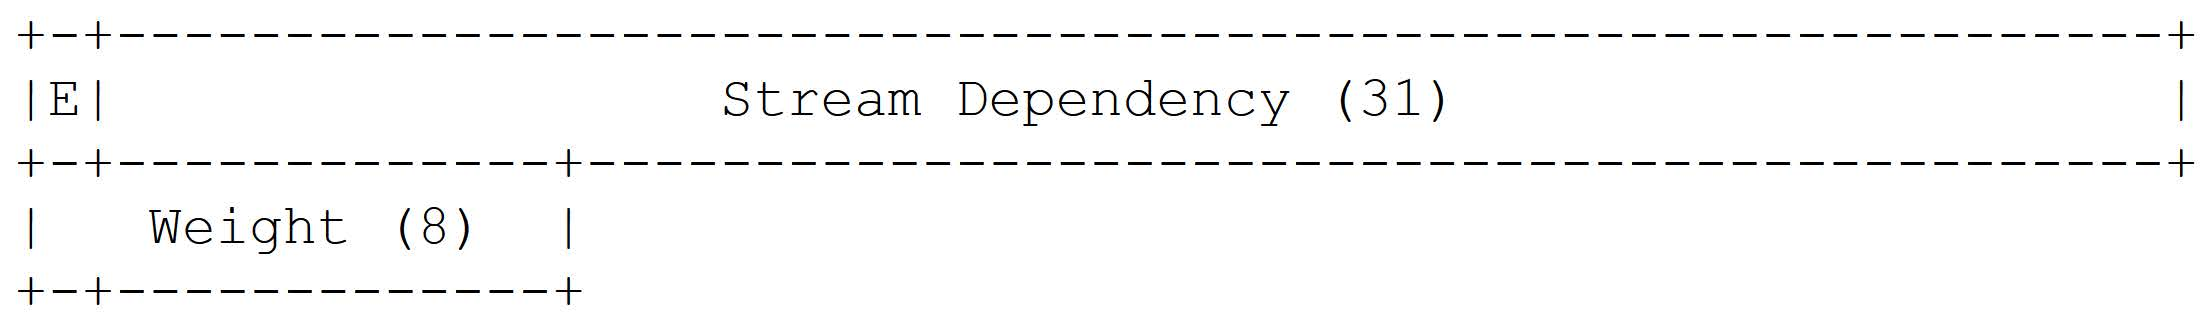
\includegraphics[width=\linewidth]{Images/Priority_frame.jpg}
	\caption{Priority frame structure}
	\label{fig:priority_frame}
\end{figure}

A \texttt{PRIORITY} frame updates the priority information for a stream. It has no flags in its frame header. Its payload contains the fields used to express the stream dependency and relative weight:

\begin{itemize}
    \item \texttt{Exclusive}: when set, it indicates that the stream should become the only child of the parent stream on which it depends.
    \item \texttt{Stream Dependency}: the identifier of the parent stream.
    \item \texttt{Weight}: the priority weight assigned to the stream.
\end{itemize}

The exclusive flag affects the structure of the prioritization tree. Without exclusivity, a new dependency can be added as another child of an existing parent. With exclusivity, the stream becomes the exclusive dependent of that parent, changing how other dependent streams are positioned in the tree. This mechanism allows the client to express not only independent weights, but also a relative ordering of resource importance.\\

A \texttt{PRIORITY} frame carries scheduling information only. It does not transfer HTTP header fields or body data, and it does not by itself create an HTTP request or response. Its role is to refine how the active streams should be served.

\section{RST\_STREAM Frames}

\begin{figure}[!h]
	\centering
	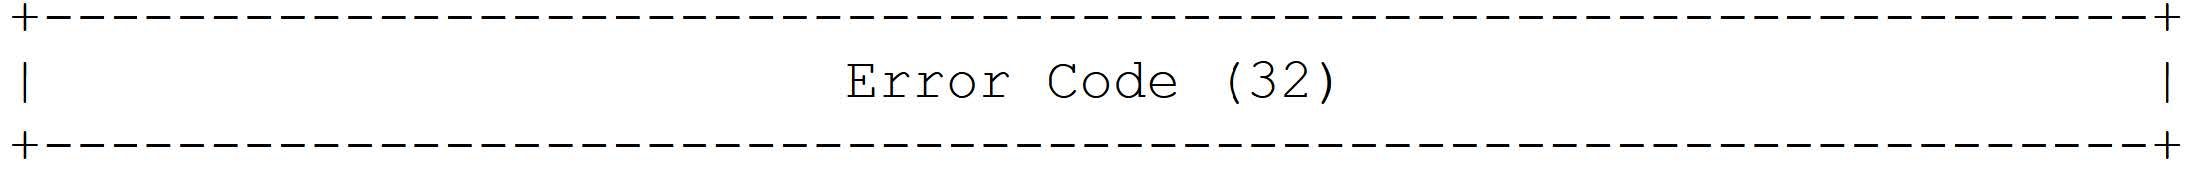
\includegraphics[width=\linewidth]{Images/RST_Stream_frame.jpg}
	\caption{RST\_Stream frame structure}
	\label{fig:RST_Stream_frame}
\end{figure}

A \texttt{RST\_STREAM} frame is used to terminate a stream immediately. Typical reasons include request cancellation, local application decisions, protocol errors, or conditions that make continuation of the stream unnecessary or invalid. For instance, if a user cancels a page load before a requested resource has been fully transferred, the client can reset the corresponding stream rather than waiting for normal completion.\\

A \texttt{RST\_STREAM} frame has no flags in its frame header. Its payload contains only a 32-bit error code. The error code identifies the condition that caused the reset. HTTP/2 defines codes for several standard situations, allowing the receiving endpoint to distinguish normal cancellation from protocol-level failures and other exceptional cases.\\

Stream reset is scoped to one stream, not necessarily to the entire connection. This distinction is important in a multiplexed protocol: terminating one exchange should not force the closure of unrelated streams that are active on the same TCP connection. By providing stream-level reset, HTTP/2 can cancel or fail individual operations while preserving the connection for other concurrent work.

\chapter{Flow Control, Server Push, and Connection Management}

\section{Flow Control in a Multiplexed Connection}

HTTP/2 multiplexing allows many streams to share the same TCP connection. This improves connection utilization, but it also introduces the risk that one endpoint may send data faster than the other endpoint can process it. Flow control is the mechanism used to prevent a sender from overwhelming a receiver with message-body bytes.\\

TCP already includes transport-level flow control, but this is not sufficient for HTTP/2. TCP flow control applies to the byte stream of the whole connection, whereas HTTP/2 needs control at the level of the logical streams multiplexed inside that connection. A receiver may be able to accept data for one stream while temporarily delaying data for another stream. Moreover, TCP flow control is below the application layer and does not expose the stream-aware control decisions needed by HTTP clients and servers.\\

HTTP/2 therefore provides its own application-layer flow control. The mechanism applies only to \texttt{DATA} frames, because these frames carry the potentially large message-body payloads. Control frames and header frames are not subject to this flow-control accounting. Flow control cannot be disabled, although endpoints can choose window sizes and update strategies according to their implementation needs.

\subsection{Flow-Control Windows}

\begin{figure}[!h]
	\centering
	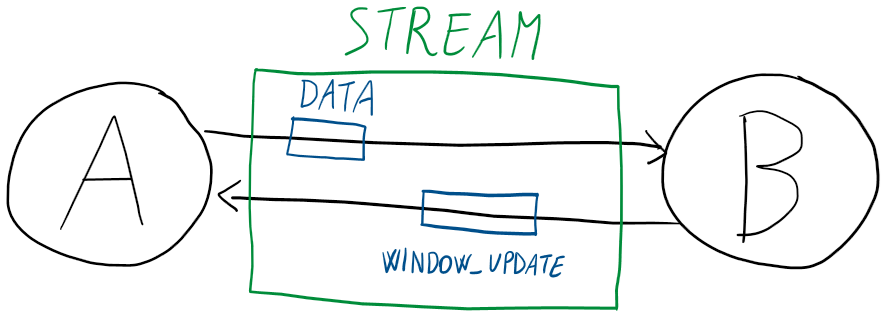
\includegraphics[width=0.6\linewidth]{Images/Window_update.png}
	\caption{Stream between A and B. A sends a DATA frame to B and B sends a WINDOW\_UPDATE frame to A.}
	\label{fig:window_update}
\end{figure}

Flow control is based on a window. The window value indicates how many additional bytes of \texttt{DATA} payload the sender is allowed to transmit before it must wait for the receiver to grant more capacity.\\

HTTP/2 maintains flow-control windows at two scopes:

\begin{itemize}
    \item a connection-level window, which limits the total amount of data in flight on the whole HTTP/2 connection;
    \item a stream-level window, which limits the amount of data in flight for each individual stream.
\end{itemize}

The initial flow-control window size is \(65{,}535\) bytes. This value applies to the connection-level window and to the initial stream-level window unless it is changed by configuration. Whenever an endpoint sends a \texttt{DATA} frame, the number of payload bytes in that frame is subtracted from the appropriate flow-control window. When the receiver is ready to accept more bytes, it increases the window by sending a \texttt{WINDOW\_UPDATE} frame.\\

Flow-control windows are directional. The amount of data that endpoint \(A\) may send to endpoint \(B\) is independent of the amount of data that \(B\) may send to \(A\). Consequently, each side manages the receive capacity it grants to the peer.\\

If a window reaches zero, the sender is not allowed to send further \texttt{DATA} frames subject to that window. The sender must wait until the receiver increases the window. This rule prevents buffering pressure at the receiving endpoint and allows the application to regulate the transfer of large bodies.

\subsection{Window Evolution Example}

Assume that the current stream-level flow-control window is \(65{,}535\) bytes. If the sender transmits a \texttt{DATA} frame carrying \(50{,}000\) bytes of payload, the remaining window becomes:

\[
65{,}535 - 50{,}000 = 15{,}535 \text{ bytes}.
\]

At this point the sender can still transmit at most \(15{,}535\) bytes on that stream before it must stop. If the receiver later sends a \texttt{WINDOW\_UPDATE} increasing the window by \(40{,}000\) bytes, the new available window becomes:

\[
15{,}535 + 40{,}000 = 55{,}535 \text{ bytes}.
\]

The update does not mean that the receiver has requested a specific object or changed the semantics of the HTTP exchange. It only grants additional sending credit for \texttt{DATA} frames. The receiver sends such updates when it has consumed or is prepared to buffer more data.\\

HTTP/2 does not mandate a specific algorithm for deciding when and by how much the receiver should update a window. Browsers, servers, and intermediaries can implement different strategies, for example updating frequently with small increments or less frequently with larger increments. The protocol specifies the frame-based mechanism, not the local policy.

\newpage
\section{\texttt{WINDOW\_UPDATE} Frames}

\begin{figure}[!h]
	\centering
	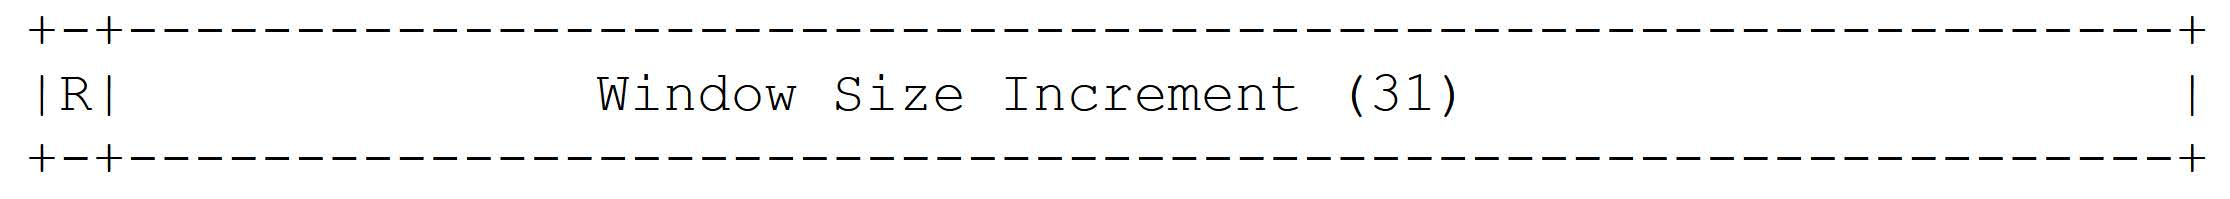
\includegraphics[width=\linewidth]{Images/Window_update_frame.jpg}
	\caption{WINDOW\_UPDATE frame structure}
	\label{fig:window_update_frame}
\end{figure}

A \texttt{WINDOW\_UPDATE} frame is the protocol object used to increase a flow-control window. It has no frame-specific flags. Its payload contains:

\begin{itemize}
    \item a reserved bit, which is not used by the flow-control algorithm;
    \item a \texttt{Window Size Increment}, which specifies the number of bytes that the sender of data is allowed to transmit in addition to the currently available window.
\end{itemize}

The stream identifier determines the scope of the update. A \texttt{WINDOW\_UPDATE} frame on stream \(0\) updates the connection-level flow-control window. A \texttt{WINDOW\_UPDATE} frame carrying a non-zero stream identifier updates the window for that stream.\\

The use of explicit updates makes the mechanism compatible with multiplexing. A receiver can grant more capacity to a specific stream without granting the same amount to all other streams, and it can also regulate the aggregate amount of data in flight across the whole connection.

\section{Server Push}

\begin{figure}[!h]
	\centering
	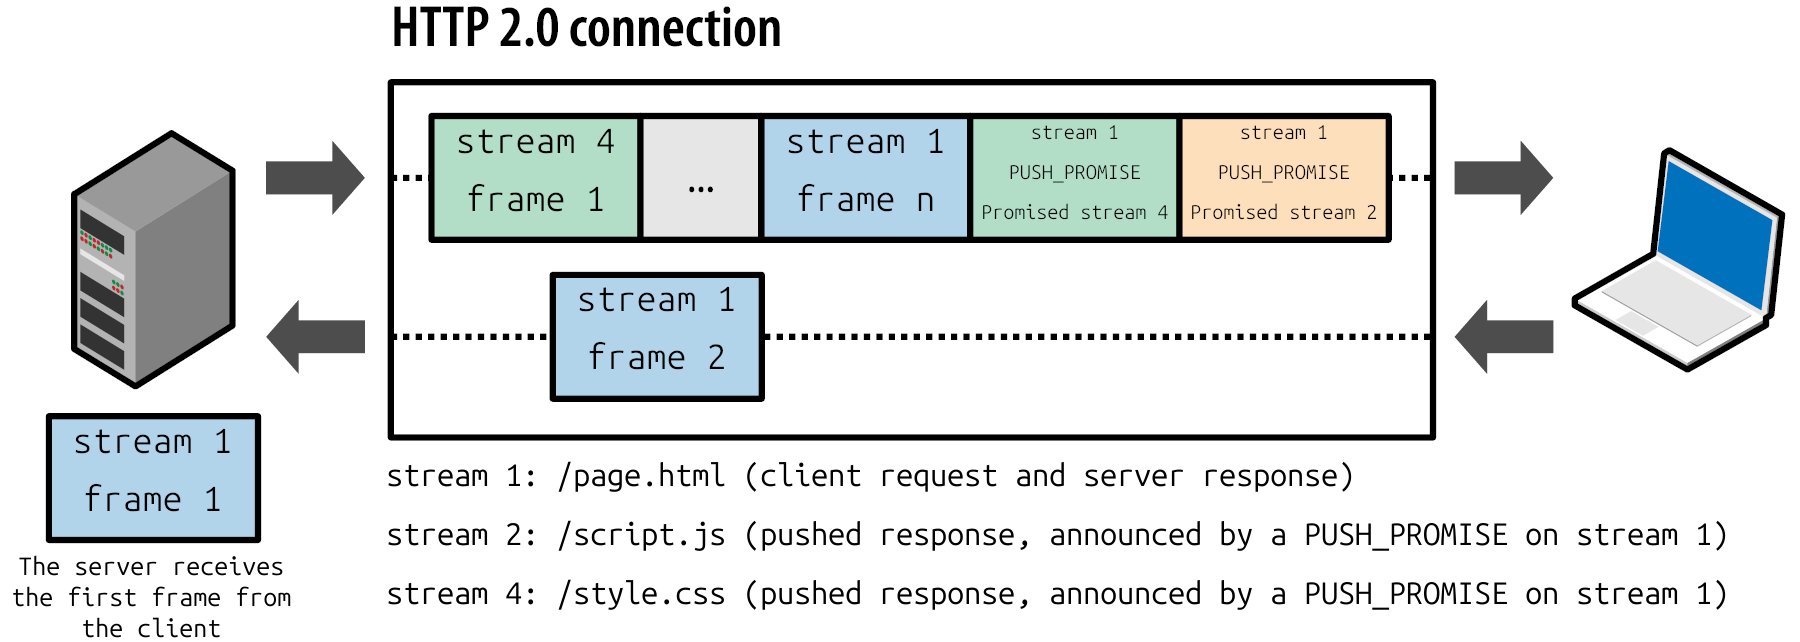
\includegraphics[width=\linewidth]{Images/Server_push.png}
	\caption{Example of HTTP 2.0 connection with server push. -- \textbf{The figure in the slides is inaccurate. This is the correct one.}}
	\label{fig:server_push}
\end{figure}

A typical web page is not limited to the initial HTML document. It normally depends on style sheets, scripts, images, fonts, and other resources. In HTTP/1.x, the client first requests the main resource, receives enough of it to discover references to subordinate resources, and then issues further requests. This discovery process introduces latency: the server may already know which resources are needed, but it must wait until the client asks for them.\\

HTTP/2 server push reduces this latency by allowing the server to send associated resources before the client has explicitly requested them. The pushed resource is not arbitrary: it must be related to a resource that the client did request. For example, after receiving a request for an HTML page, the server may infer that the corresponding style sheet or script will be needed and can start the push process while the original response is still being transferred.\\

Server push preserves HTTP semantics by making the pushed response correspond to a request that the server promises on behalf of the client. The server does not simply inject bytes into the connection without structure; it first announces the intended pushed stream and then sends a regular HTTP response on that stream.\\

Let us look at figure \ref{fig:server_push} to have an example of HTTP 2.0 connection with server push. The client sends the server the first frame of the first stream and the server receives it. Considering that in the HTTP/2 protocol the client doesn't have to wait for the server response before sending another frame, the former sends the second frame of the first stream.\\

When the server receives the first message of the first stream, it processes the received request and understands that it has to send the requested resource \texttt{/page.html} to the client and, considering that the page has related resources, it announces the client that it will send other two resources on a separate stream each.\\

Remember that the streams initiated by the server have an even number while the ones initialized by the client have an odd number to reflect the client-server model in which the client sends the $1^{st}$ message (1 is an odd number) and the server sends the $2^{nd}$ message (2 is an even number). Also remember that the stream numbers are assigned in ascending order so, the first stream announced by the server must have a smaller number than the second.\\

In this example the stream related to the file \texttt{/script.js} has number 2 and the stream related to the file \texttt{/style.css} has number 4.\\

What really matters to the end of the correctness of the transmission is that the promise of one stream is prior to the stream itself. The fact that in the picture the response to the user's request (stream 1 frame n) is transmitted after the promises does not mean that the responses are necessarily transmitted after the promises. The response could have also been transmitted first or between the promises.

\subsection{Properties of Pushed Resources}

Pushed resources can participate in the same mechanisms as ordinary resources:

\begin{itemize}
    \item they can be cached by the client if the usual HTTP caching rules allow it;
    \item they can be reused across different pages when the cache entry is valid;
    \item they can be multiplexed with other streams on the same connection;
    \item they can be prioritized by the server together with requested resources;
    \item they can be declined by the client when the push is unnecessary or unwanted.
\end{itemize}

The ability to decline pushed resources is important because the server does not have perfect knowledge of the client's state. The client may already have a fresh cached copy, may not need the resource because of application state, or may choose to reject server push according to local policy.

\subsection{Relationship with Multiplexing}

Server push relies on the same stream and frame abstraction used for ordinary requests and responses. This is essential for efficiency. A pushed resource does not require a new TCP connection and does not block the explicitly requested response. Its frames can be interleaved with frames belonging to the original stream and with frames from other concurrent streams.\\

The benefit is strongest when the server can predict the resources needed by the client before the client would otherwise discover them. Incorrect prediction can waste bandwidth, so practical use of server push requires careful selection of resources, attention to cacheability, and coordination with prioritization.

\section{\texttt{PUSH\_PROMISE} Frames}

A \texttt{PUSH\_PROMISE} frame notifies the receiver in advance that the sender intends to initiate a pushed stream. The frame is sent on the stream associated with the explicitly requested resource. Its role is to reserve a new server-initiated stream and to describe the request headers that the server assumes for the pushed resource.\\

A push promise therefore has two related stream identities:

\begin{itemize}
    \item the stream on which the \texttt{PUSH\_PROMISE} frame is sent, corresponding to the request that caused the push opportunity;
    \item the promised stream identifier, corresponding to the new stream on which the pushed response will later be sent.
\end{itemize}

The header block carried by the promise contains the HTTP request header fields that the server considers applicable to the pushed resource. Conceptually, the promise says that the server is about to send a response as if the client had made that request.

\subsection{Flags}

A \texttt{PUSH\_PROMISE} frame defines the following flags:

\begin{itemize}
    \item \texttt{END\_HEADERS} (\texttt{0x4}): when set, the frame contains the complete header block and is not followed by \texttt{CONTINUATION} frames for the same header block.
    \item \texttt{PADDED} (\texttt{0x8}): when set, the payload includes a pad-length field and padding bytes.
\end{itemize}

If the promised request header block does not fit in one frame, it can be continued with \texttt{CONTINUATION} frames on the same associated stream. These continuation frames extend the promise header block; they are not the response to the pushed resource.

\newpage
\subsection{Payload Structure}

\begin{figure}[!h]
	\centering
	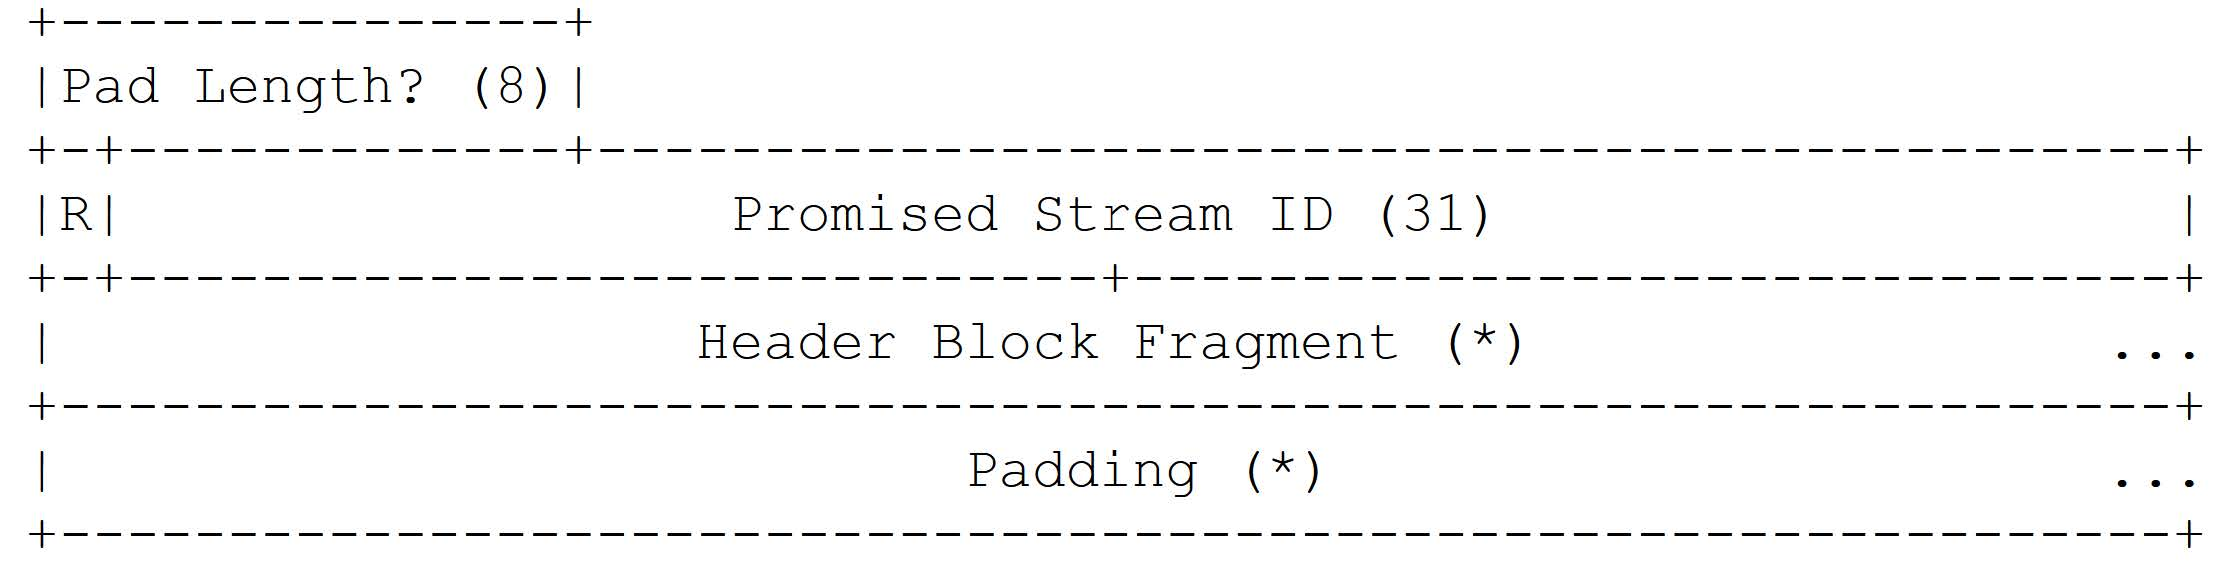
\includegraphics[width=\linewidth]{Images/Push_promise_frame_payload.jpg}
	\caption{PUSH\_PROMISE frame payload}
	\label{fig:push_promise_frame_payload}
\end{figure}

The payload of a \texttt{PUSH\_PROMISE} frame may contain (see figure \ref{fig:push_promise_frame_payload}):

\begin{itemize}
    \item \texttt{Pad Length}, present only when \texttt{PADDED} is set;
    \item a reserved bit;
    \item \texttt{Promised Stream ID}, the identifier of the server-initiated stream reserved by the promise;
    \item \texttt{Header Block Fragment}, containing the compressed header block fragment for the promised request;
    \item \texttt{Padding}, present only when \texttt{PADDED} is set.
\end{itemize}

After the promise has been accepted, the pushed response is transmitted on the promised stream using the same representation as an ordinary response: header fields in \texttt{HEADERS} frames and body bytes in \texttt{DATA} frames. The difference is not in the response format, but in how the stream was initiated.

\section{Connection Testing with \texttt{PING}}

\begin{figure}[!h]
	\centering
	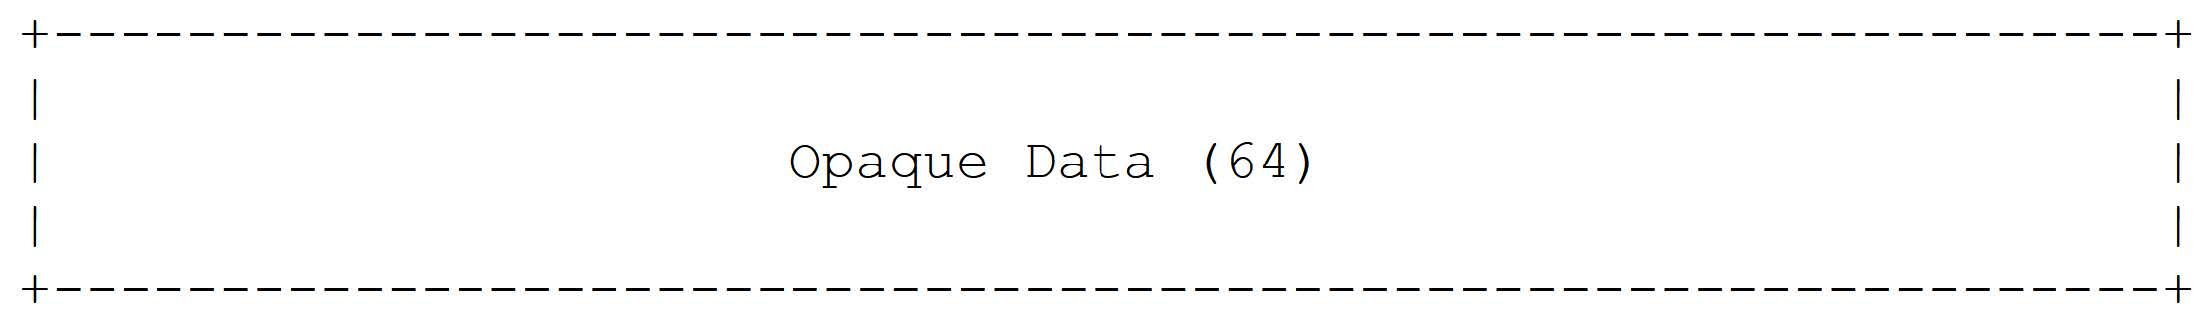
\includegraphics[width=\linewidth]{Images/Ping_frame.jpg}
	\caption{Ping frame payload}
	\label{fig:ping_frame}
\end{figure}

A \texttt{PING} frame is used to test whether an idle connection is still functional and to measure round-trip time. It is a connection-level frame and is not associated with an individual request-response stream.\\

The payload consists of exactly \(8\) bytes of opaque data. The receiver echoes the opaque data in the corresponding acknowledgement, allowing the sender to match the response to the original probe and compute an approximate round-trip time. Since the payload is opaque, the protocol does not assign application semantics to those bytes.\\

The frame is useful in long-lived connections where the absence of application traffic does not necessarily imply that the connection is unusable. It allows an endpoint to distinguish an idle but alive connection from a broken one without creating an artificial HTTP request.

\section{Connection Shutdown with \texttt{GOAWAY}}

\begin{figure}[!h]
	\centering
	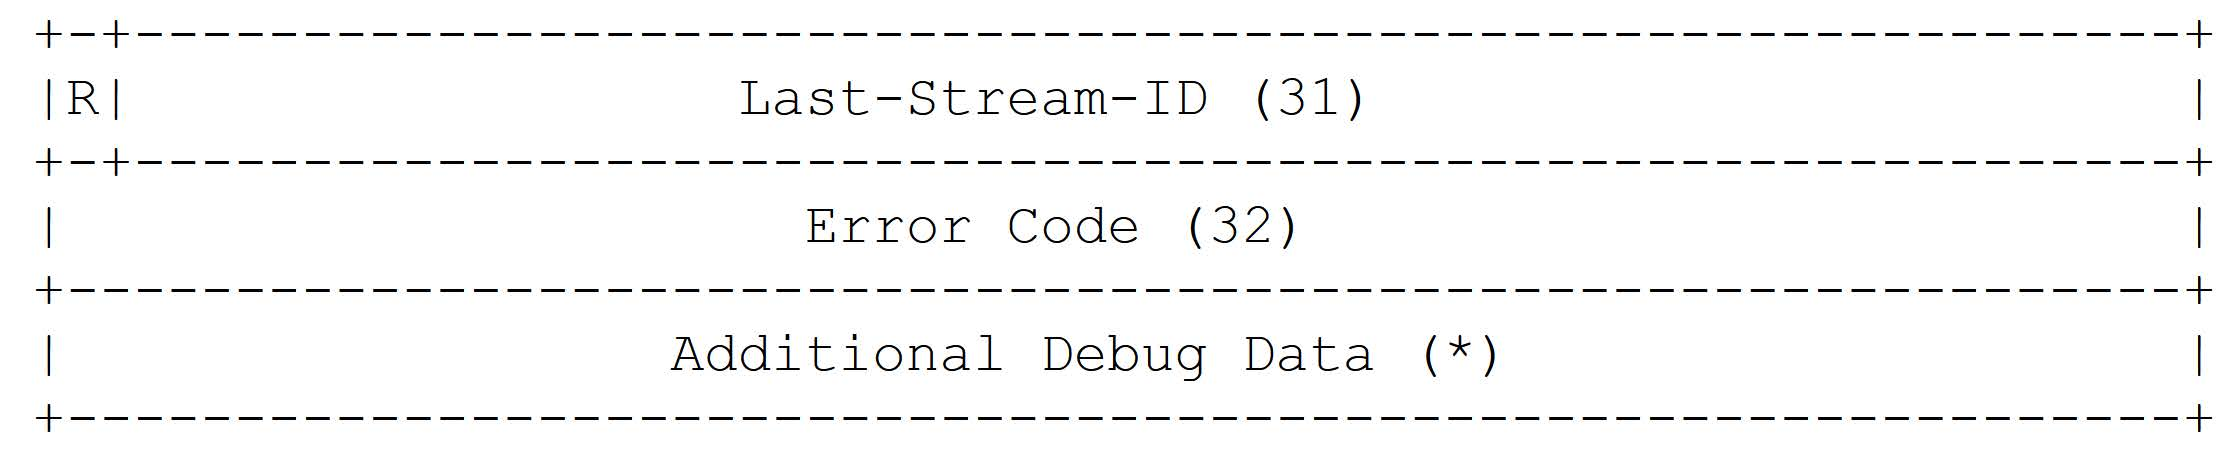
\includegraphics[width=\linewidth]{Images/Goaway_frame_payload.jpg}
	\caption{GOAWAY frame payload}
	\label{fig:goaway_frame_payload}
\end{figure}

A \texttt{GOAWAY} frame initiates shutdown of an HTTP/2 connection. It is scoped to the connection as a whole rather than to a single stream. This distinction separates connection termination from stream termination: \texttt{RST\_STREAM} closes one stream, whereas \texttt{GOAWAY} starts closing the connection.\\

A \texttt{GOAWAY} frame has no frame-specific flags. Its payload contains:

\begin{itemize}
    \item a reserved bit;
    \item \texttt{Last Stream ID}, the highest-numbered stream identifier that the sender of the \texttt{GOAWAY} might have processed;
    \item \texttt{Error Code}, using the same error-code space as stream errors;
    \item optional \texttt{Additional Debug Data}, whose content is opaque to the protocol.
\end{itemize}

The \texttt{Last Stream ID} field is necessary because streams may be active or in the process of being created when shutdown begins. By stating the highest stream it might have processed, the sender gives the peer enough information to determine which streams may need to be retried on a different connection.\\

The error code is present because \texttt{GOAWAY} is used both for graceful shutdown and for error cases. In a normal termination, the endpoint can indicate that no protocol error caused the shutdown. In an exceptional termination, the error code communicates the reason for closing the connection.

\newpage
\section{Connection Configuration with \texttt{SETTINGS}}

\begin{figure}[!h]
	\centering
	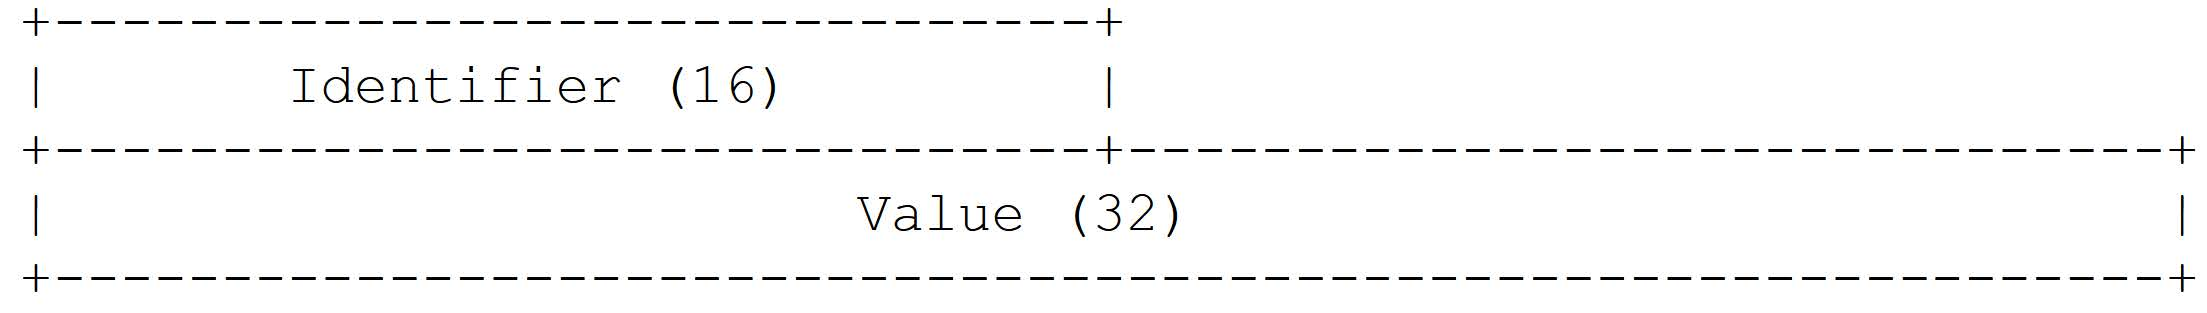
\includegraphics[width=\linewidth]{Images/Settings_frame_payload.jpg}
	\caption{SETTINGS frame payload}
	\label{fig:settings_frame_payload}
\end{figure}

A \texttt{SETTINGS} frame is used to exchange configuration parameters that affect the behavior of the HTTP/2 connection. These settings are not HTTP header fields and are not part of any individual request or response. They define protocol-level constraints and preferences for the connection.\\

A \texttt{SETTINGS} frame contains zero or more parameter pairs. Each pair consists of:

\begin{itemize}
    \item a 16-bit setting identifier;
    \item a 32-bit value.
\end{itemize}

Settings are acknowledged. A \texttt{SETTINGS} frame with the \texttt{ACK} flag set acknowledges that the receiver has received and applied a previous \texttt{SETTINGS} frame. An acknowledgement frame must have an empty payload, because it does not introduce new parameters; it only confirms application of earlier ones.

\subsection{Selected Settings}

Several settings are especially relevant to the mechanisms discussed in this chapter:

\begin{description}
    \item[\texttt{SETTINGS\_ENABLE\_PUSH}] controls whether the peer is allowed to use server push. Disabling this setting lets a client prevent the server from initiating pushed streams.
    \item[\texttt{SETTINGS\_MAX\_CONCURRENT\_STREAMS}] specifies the maximum number of concurrent streams that the sender allows the receiver to create. This bounds multiplexing and prevents uncontrolled growth of active stream state.
    \item[\texttt{SETTINGS\_INITIAL\_WINDOW\_SIZE}] specifies the initial stream-level flow-control window size, in bytes. The default value is \(65{,}535\) bytes.
    \item[\texttt{SETTINGS\_MAX\_FRAME\_SIZE}] specifies the maximum frame payload size acceptable to the sender. The default value is \(16{,}384\) bytes, and the value cannot exceed \(2^{24}-1\) bytes.
\end{description}

These settings show that HTTP/2 behavior is partly negotiated at connection setup and can be adapted to endpoint capabilities. A server may restrict concurrency to protect memory and CPU resources; a client may disable push to avoid unnecessary bandwidth usage; either endpoint may adjust flow-control parameters to match its buffering strategy.

\section{Operational Interaction of the Mechanisms}

Flow control, server push, and connection management are separate mechanisms, but they interact during normal operation. A pushed response is transmitted as \texttt{DATA} frames and is therefore subject to the same flow-control windows as an explicitly requested response. A connection with too many active pushed and requested streams can be constrained by \texttt{SETTINGS\_MAX\_CONCURRENT\_STREAMS}. If the connection is being closed, \texttt{GOAWAY} indicates which streams may have been processed and which should not be assumed to have completed.\\

The common design principle is that each mechanism preserves multiplexing without losing control. \texttt{WINDOW\_UPDATE} regulates data volume, \texttt{PUSH\_PROMISE} introduces anticipated resources in a structured way, \texttt{PING} tests connection liveness, \texttt{GOAWAY} shuts down the connection without confusing stream state, and \texttt{SETTINGS} defines the parameters under which the connection operates.

\chapter{HTTP/2 Header Compression and Protocol Negotiation}

\section{Motivation for Header Compression}

\begin{figure}[!h]
	\centering
	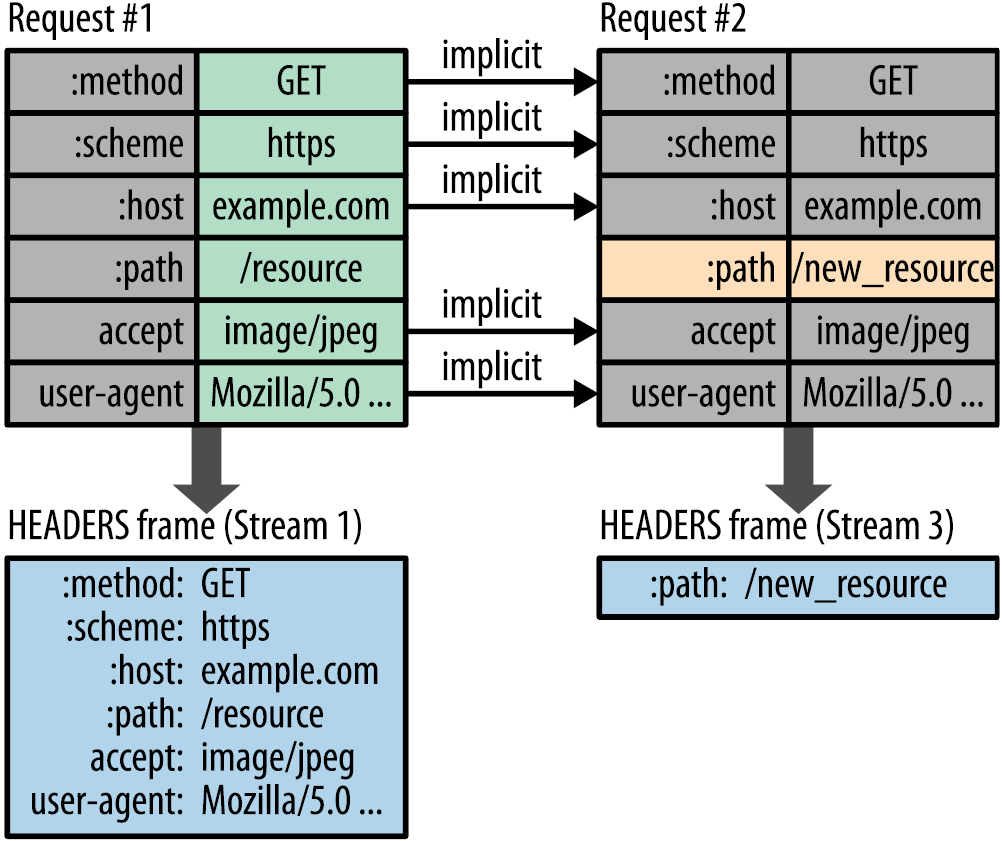
\includegraphics[width=0.6\linewidth]{Images/Header_compression.png}
	\caption{Figure showing two requests made to the same server. In the first request all the header fields are explicit because they are unknown to the communicating parts. In the second request, the client does not need to transmit again the previously sent headers and need to transmit only the different one which, in this case, is the path of the requested resource.}
	\label{fig:header_compression}
\end{figure}

HTTP/2 preserves the semantics of HTTP messages while replacing their textual transfer representation with binary frames. This change is especially relevant for header fields. In HTTP/1.x, headers are transmitted as plain text in every request and response. Many of them are repetitive across requests to the same origin: cookies, accepted formats, user-agent information, cache validators, authentication metadata, and other fields often change little or not at all during a browsing session.\\

When a page requires many resources, repeated headers can represent a significant fraction of the bytes exchanged before the useful payload is delivered. This effect is particularly visible for small resources, where the body may be much smaller than the repeated metadata that accompanies the request. HTTP/2 addresses this overhead by encoding request and response header fields with the HPACK compression algorithm.\\

Header compression is not an optional optimization placed outside the protocol. It is part of the HTTP/2 message representation. A logical HTTP header block is converted into a compact binary form and carried inside frame payloads, mainly \texttt{HEADERS}, \texttt{PUSH\_PROMISE}, and, when necessary, \texttt{CONTINUATION} frames. The receiver decodes the header block and reconstructs the usual HTTP fields before delivering the message to the application logic.

\section{The HPACK Compression Model}

HPACK is the header compression format defined for HTTP/2. Its role is to reduce the cost of transmitting HTTP header fields while preserving their meaning. The algorithm combines two complementary mechanisms:

\begin{itemize}
    \item a static coding mechanism, based on a predefined Huffman code table;
    \item a shared compression context, maintained by both endpoints, that records previously seen header fields and makes repeated values cheap to encode.
\end{itemize}

The result is a representation in which common and repeated headers can be transmitted using short binary references rather than full textual field names and values. HPACK operates on header fields, not on message bodies. Payload bytes are carried by \texttt{DATA} frames and are not compressed by HPACK.

\subsection{Static Huffman Coding}

HPACK includes a static Huffman code table. The table is fixed by the specification, so the encoder and decoder do not need to negotiate or transmit the coding dictionary during the connection. A string can therefore be represented using a compact sequence of bits according to a code that both endpoints already know.\\

This mechanism is useful for compressing individual header names and values, especially when they contain characters and substrings that occur frequently in HTTP metadata. Since the coding table is static, decoding does not depend on previous messages and does not require synchronization beyond the normal HPACK decoding rules.\\

The static Huffman code is not the whole compression algorithm. It compresses strings, while the table-based mechanisms described below exploit repetition at the level of complete header fields and header values.

\subsection{Static and Dynamic Header Tables}

HPACK represents header fields using tables. A table entry can contain a complete name-value pair, or it can help encode a field by reusing a known name while transmitting a new value.\\

The static table contains common HTTP header names and frequent name-value combinations. Since this table is predefined, both endpoints can refer to its entries by index without transmitting the full strings. For example, frequently used field names such as \texttt{:method}, \texttt{:path}, \texttt{:status}, \texttt{content-type}, or \texttt{cache-control} are suitable for indexed representation because they occur repeatedly in normal HTTP traffic.\\

The dynamic table is the part of the compression context that changes during the connection. Client and server maintain synchronized views of this table. When an endpoint sends a header field that is likely to recur, it may insert that field into the dynamic table. Later header blocks can then refer to the same field, or to the same field name, using a compact index.\\

This shared context is effective because HTTP traffic to the same origin is highly repetitive. A first request may need to encode a field explicitly; a later request can often encode the same field with an index. Consider the following simplified sequence of requests:

\begin{lstlisting}
GET /index.html HTTP/1.1
Host: server.example.com
User-Agent: ExampleBrowser
Accept: text/html
Cookie: session=abc123

GET /style.css HTTP/1.1
Host: server.example.com
User-Agent: ExampleBrowser
Accept: text/css
Cookie: session=abc123
\end{lstlisting}

The two requests differ in the requested path and accepted media type, but several fields are repeated. HPACK can exploit this repetition by representing already known fields with references rather than retransmitting their full textual form. The application still sees ordinary HTTP headers after decoding; only the wire representation is compressed.

\subsection{Indexed and Literal Representations}

HPACK does not require every header field to be transmitted in the same form. Depending on the field and on the state of the compression context, an encoder may choose among different representations.\\

An indexed representation refers to a complete table entry. This is the most compact case: the encoded header field says, in effect, that the field is identical to an entry already known to both endpoints. A literal representation transmits a new value, possibly reusing a known field name from the table. A literal field may also be inserted into the dynamic table so that later header blocks can refer to it.\\

The choice is implementation-dependent. Fields that are stable and repeated are good candidates for indexing. Fields that are large, volatile, or sensitive may be encoded without insertion into the dynamic table. This distinction prevents the compression context from being polluted by values that are unlikely to be reused and gives implementations control over memory usage and exposure of sensitive metadata.

\section{Header Blocks in HTTP/2 Frames}

An HTTP/2 header block is the compressed representation of the header section of an HTTP request or response. It is not necessarily carried in a single frame. The first fragment of a header block is carried by a frame that introduces headers, typically \texttt{HEADERS} for ordinary requests and responses or \texttt{PUSH\_PROMISE} for server push. If the header block does not fit in that frame, the remaining fragments are carried by one or more \texttt{CONTINUATION} frames.\\

The \texttt{END\_HEADERS} flag indicates the end of the header block. When this flag is set on a \texttt{HEADERS} or \texttt{PUSH\_PROMISE} frame, no \texttt{CONTINUATION} frame follows for that header block. When it is not set, the receiver continues reading \texttt{CONTINUATION} frames until the header block is complete.\\

This design separates header compression from message-body transfer. A request or response header section is compressed as one logical block, even if that block is split across multiple frames for transmission. The message body, if present, is then carried separately in \texttt{DATA} frames.

\subsection{Compression Context and Ordering}

The dynamic table makes header compression stateful. Because table updates must be interpreted in the same order by encoder and decoder, header block processing is ordered within the HTTP/2 connection. A receiver must decode header blocks consistently with the sequence of dynamic table updates that preceded them.\\

This requirement does not remove multiplexing. Frames belonging to different streams may still be interleaved on the same connection. However, compressed header blocks are decoded according to the HPACK context shared by the endpoints. Correct decoding depends on maintaining the same view of the dynamic table on both sides.\\

The implication for implementations is that header compression is part of the connection state, not an isolated transformation applied independently to each stream. This is one reason why HTTP/2 frames contain explicit stream identifiers while header compression itself is managed at the connection level.

\section{Protocol Negotiation and Upgrade}

HTTP/2 is not backward compatible with HTTP/1.x at the wire level. A server expecting an HTTP/1.1 textual request cannot directly interpret an HTTP/2 binary frame sequence, and an HTTP/2 endpoint cannot treat an HTTP/1.1 message as if it were already framed. Therefore, client and server must agree on the protocol version before exchanging HTTP/2 frames.\\

The negotiation procedure depends on whether the connection is cleartext or protected by TLS. In both cases, the goal is the same: avoid sending HTTP/2 frames to an endpoint that only understands HTTP/1.1, while allowing capable endpoints to switch to the binary framing layer.

\subsection{Cleartext Upgrade with \texttt{h2c}}

When a client makes a request to an \texttt{http} URI and has no prior knowledge that the server supports HTTP/2, it can use the HTTP/1.1 \texttt{Upgrade} mechanism. The request is initially a valid HTTP/1.1 request, so an HTTP/1.1-only server can still process or ignore it safely.\\

A typical cleartext upgrade request has the following form:

\begin{lstlisting}
GET / HTTP/1.1
Host: server.example.com
Connection: Upgrade, HTTP2-Settings
Upgrade: h2c
HTTP2-Settings: <base64url encoding of HTTP/2 SETTINGS payload>
\end{lstlisting}

The \texttt{Connection: Upgrade, HTTP2-Settings} field marks \texttt{Upgrade} and \texttt{HTTP2-Settings} as connection-specific fields. The \texttt{Upgrade: h2c} field identifies HTTP/2 over cleartext TCP as the requested protocol. The \texttt{HTTP2-Settings} field carries a base64url-encoded HTTP/2 \texttt{SETTINGS} payload, allowing the client to provide its initial HTTP/2 configuration as part of the upgrade request.\\

If the server supports the requested protocol and accepts the upgrade, it responds with status code \texttt{101 Switching Protocols}:

\begin{lstlisting}
HTTP/1.1 101 Switching Protocols
Connection: Upgrade
Upgrade: h2c

[ HTTP/2 connection ...
\end{lstlisting}

After this response, the connection changes protocol. The subsequent bytes belong to the HTTP/2 connection and are interpreted according to the binary framing layer. The exchange that initiated the upgrade is then completed using HTTP/2 semantics on the upgraded connection.\\

If the server does not support HTTP/2, it can ignore the upgrade request and respond as if the \texttt{Upgrade} field were absent. This behavior preserves compatibility: the client has sent a syntactically valid HTTP/1.1 request, and the server is not forced to understand HTTP/2 in order to respond.

\subsection{HTTP/2 over TLS}

The protocol identifier \texttt{h2} denotes HTTP/2 over TLS, while \texttt{h2c} denotes HTTP/2 over cleartext TCP. In secure deployments, protocol selection is performed before HTTP messages are exchanged, during TLS negotiation. Once both endpoints have selected \texttt{h2}, the application-layer traffic carried by the TLS connection is HTTP/2 traffic rather than HTTP/1.1 textual messages.\\

This distinction is operationally important. With cleartext \texttt{http}, the client can begin with an HTTP/1.1 request and ask to upgrade the existing connection. With \texttt{https}, the protocol must be selected inside the secure connection setup so that both endpoints agree on how to interpret the protected application data. After negotiation, HTTP semantics remain unchanged, but requests and responses are encoded as HTTP/2 frames and header fields are compressed with HPACK.

\section{Interaction Between Compression and Negotiation}

Negotiation determines whether the connection will use HTTP/2 at all. Header compression determines how HTTP metadata is represented once HTTP/2 has been selected. The two mechanisms are therefore sequential in normal operation: the endpoints first agree on HTTP/2 support, then they exchange connection settings and begin transmitting compressed header blocks inside frames.\\

A successful negotiation does not require web applications to change their use of HTTP methods, status codes, URIs, or header fields. The transformation occurs below the application-visible HTTP semantics. For the application, a request still has fields such as \texttt{:method}, \texttt{:path}, \texttt{host}-related authority information, content negotiation metadata, and optional body data. For the connection, the same information is represented as binary frames containing HPACK-compressed header blocks and, when needed, \texttt{DATA} frames.\\

The combination of binary framing, multiplexing, flow control, prioritization, server push, and HPACK compression defines the operational profile of HTTP/2. Multiplexing reduces the need for multiple TCP connections. Flow control prevents one endpoint from overwhelming the other. Prioritization lets the client express relative resource importance. Server push allows anticipated resources to be associated with an explicit request. HPACK reduces the overhead of repetitive metadata. Protocol negotiation ensures that these mechanisms are used only when both endpoints understand them.

\end{document}